\documentclass[11pt]{article}

\usepackage[T1]{fontenc}
\usepackage[margin=1.15in]{geometry}
\usepackage{amsmath,amssymb,amsthm}
\usepackage{booktabs}
\usepackage{array}
\usepackage{enumitem}
\usepackage{tikz}
\usepackage[colorlinks=true,linkcolor=black,citecolor=black,urlcolor=black]{hyperref}

\setlength{\parskip}{0.5em}
\setlength{\parindent}{0pt}
\renewcommand{\arraystretch}{1.25}

\newtheorem{theorem}{Theorem}[section]
\newtheorem{proposition}[theorem]{Proposition}
\newtheorem{lemma}[theorem]{Lemma}
\newtheorem{corollary}[theorem]{Corollary}
\theoremstyle{definition}
\newtheorem{definition}[theorem]{Definition}
\newtheorem{example}[theorem]{Example}
\theoremstyle{remark}
\newtheorem{remark}[theorem]{Remark}

\newcommand{\R}{\mathbb{R}}
\newcommand{\Rop}{\mathcal{R}}
\newcommand{\dox}[1]{\mathrm{do}(#1)}
\newcommand{\ind}{\mathbf{1}}
\DeclareMathOperator{\argmin}{arg\,min}

\title{\textbf{Ablation Invariance}\\[0.4em]
\large What Null Ablations Reveal About Hidden Architecture}
\author{Flyxion\\Independent Researcher}
\date{September 2026}

\begin{document}
\maketitle

\begin{abstract}
\noindent
The experimental sentence ``we removed $C$, and nothing happened'' is usually read as evidence that $C$ is unimportant. This essay argues that the sentence supports far less than that, and that in many cases it supports something more interesting. A null ablation certifies only that one finite intervention, applied under specific conditions and read through one observable, failed to move that observable. It does not establish that the sensitivity $\partial O/\partial C$ vanishes, that $C$ is dispensable, or that the system after the intervention is the system with $C$ subtracted. Adaptive, redundant, and degenerate systems answer an ablation by reconfiguring, so the object actually measured is $\Rop(S,\dox{C=0})$ and not $S-C$. We give a formal treatment of this gap. We separate component necessity from path necessity, define a compensation gap that lower-bounds hidden rerouting, prove that single-ablation nulls are compatible with exponentially many distinct architectures, show that joint ablations expose the interaction structure that singles conceal, and prove that the same nulls become fully informative once the observable is enriched from a scalar to a residual vector. The last result outlines a form of structural tomography in which sequences of ablations and their compensations reconstruct an invisible network. Invariance is reframed as change confined to a fibre of the observation map, so that a null ablation reports motion within the observational quotient and not the absence of motion, and the null is shown to be compatible with unchanged output at nonzero cost and reduced margin. A minimal reporting standard is proposed.
\end{abstract}

\tableofcontents
\newpage

%------------------------------------------------------------------
\section{The Statement}
%------------------------------------------------------------------

Consider the sentence
\begin{quote}
\emph{We removed $C$, and nothing happened.}
\end{quote}
It appears, in one form or another, in ablation studies of neural networks, in gene knockout papers, in lesion neuroscience, in engineering inspections, in institutional reform, and in ordinary household repair. The sentence is usually followed by an inference: $C$ was not doing anything, or at least nothing that mattered. The inference is so habitual that it is rarely written down, which is a reason to write it down and examine it.

Three distinct objects are being run together in the sentence. The first is the \emph{finite intervention} $\dox{C=0}$: a specific act performed on a specific system at a specific time, replacing the state or parameters of $C$ by a null value. The second is the \emph{sensitivity} $\partial O/\partial C$: a local property of the response of an observable $O$ to changes in $C$ around some operating point. The third is the \emph{measured observable} $O$ itself, which is one projection of the system's behavior, taken at one resolution, under one set of conditions. The inference from ``nothing happened'' to ``$C$ is irrelevant'' silently identifies the first with the second and treats the third as exhaustive.

The central proposition of this essay is that the identification fails:
\begin{equation}\label{eq:central}
\Delta O \approx 0 \quad\not\Rightarrow\quad \frac{\partial O}{\partial C}=0 .
\end{equation}
Removing component $C$ and observing essentially no change in output $O$ does not establish that $C$ was causally irrelevant. It establishes that the intervention $\dox{C=0}$ did not move the measured observable under the tested conditions. Compensation by another pathway, saturation, degeneracy, coarse measurement, or redistribution of load can each make the intervention observationally silent.

Even the weakest reading of \eqref{eq:central}, that a finite change need not reflect a derivative, is worth stating with a concrete case.

\begin{example}[Finite null, nonzero derivative]\label{ex:sin}
Let $O(c)=\sin(2\pi c)$ with baseline $c=1$ and ablated value $c=0$. Then $O(1)=O(0)=0$, so $\Delta O=0$ exactly. Yet $\partial O/\partial c=2\pi\cos(2\pi c)$ equals $2\pi$ at both the baseline and the ablated point. The intervention landed on another point of the same level set of $O$.
\end{example}

This example is artificial, but it isolates the logical structure: a finite intervention compares two points, and two points can share an observable value while the function is steep at both. The interesting cases are those in which the coincidence is not an accident of periodicity but a consequence of how the system is built. In those cases the null result is not an absence of information. It is evidence about architecture.

The plan of the essay is as follows. Section~\ref{sec:setting} fixes the formal setting, including an operator $\Rop$ that models the system's own response to being ablated. Section~\ref{sec:readings} distinguishes four readings of a null ablation, and Section~\ref{sec:silence} catalogues the sources of silence. Sections~\ref{sec:geometry} and~\ref{sec:quotient} give these sources a single geometric form: a null ablation is a return to the same observational fibre, and an experiment observes only the quotient of configuration space by that relation. Section~\ref{sec:necessity} separates component necessity from path necessity and proves the main gap between $S-C$ and $\Rop(S,\dox{C=0})$. Section~\ref{sec:time} treats the adaptation horizon and shows that a null at one horizon is a quantitative bound on the system's adaptation rate. Section~\ref{sec:cost} shows that output invariance can coexist with a permanent compensation cost. Section~\ref{sec:joint} shows how joint ablations expose interaction, and Section~\ref{sec:profile} extends this to whole ablation profiles, redundancy margins, and the sampling failure of random ablation. Section~\ref{sec:slack} shows that a null can coexist with consumed reserve and reduced distance to failure. Section~\ref{sec:ident} proves that single-ablation nulls are compatible with exponentially many architectures. Section~\ref{sec:converse} treats the converse, since a non-null result is equally over-read. Section~\ref{sec:restore} introduces the rebound test, which certifies compensation without a second ablation. Section~\ref{sec:graded} treats graded interventions and shows that a zero derivative is no more decisive than a null endpoint. Section~\ref{sec:stat} gives the statistical conditions under which a null can be certified at all. Sections~\ref{sec:practice}, \ref{sec:design} and~\ref{sec:framework} draw consequences for reporting, for the design of systems and experiments, and for a broader family of frameworks, and Section~\ref{sec:objections} answers likely objections. Section~\ref{sec:observer} states the order relation among observers that underlies the resolution results, Section~\ref{sec:tomography} proves that enriching the observable turns the same nulls into a reconstruction method, and Section~\ref{sec:principle} states the general principle of preserved distinctions.

%------------------------------------------------------------------
\section{Formal Setting}\label{sec:setting}
%------------------------------------------------------------------

\subsection{Systems, interventions, observables}

Let $K=\{1,\dots,n\}$ index the components of a system. Each component $c\in K$ has a configuration space $\Theta_c$ with a distinguished null value $0_c\in\Theta_c$. The joint configuration space is $\Theta=\prod_{c\in K}\Theta_c$. For $C\subseteq K$ write $\theta=(\theta_C,\theta_{-C})$ for the decomposition of a configuration into the coordinates in $C$ and the rest.

\begin{definition}[Observable and tolerance]
An observable is a map $O:\Theta\to(Y,d)$ into a metric space. A tolerance $\varepsilon\ge 0$ is fixed in advance and encodes both measurement resolution and the smallest change regarded as meaningful. A change is $\varepsilon$-null if $d\le\varepsilon$.
\end{definition}

\begin{definition}[Ablation]
The intervention $\dox{C=0}$ sets $\theta_C:=0_C$ and holds it there. Following the usual convention of intervention calculus~\cite{pearl2009}, the intervention overrides whatever mechanism ordinarily determined $\theta_C$.
\end{definition}

The definition so far describes a static system. Real systems adapt. A neural network can be retrained or can re-route activations through other layers at inference time, an organism can upregulate paralogs, a structure can redistribute stress, and an institution can reassign duties. To capture this we attach an adaptation dynamics.

\begin{definition}[Adaptive system]\label{def:adaptive}
An adaptive system is a triple $(\Theta,V,O)$ where $V$ is a vector field on $\Theta$ (the adaptation dynamics) and $O$ is an observable. The baseline configuration $\theta^0$ is a rest point: $V(\theta^0)=0$. Under the intervention $a=\dox{C=0}$ the coordinates $\theta_C$ are pinned at $0_C$ and the free coordinates evolve by the restricted flow
\[
\dot\theta_{-C}=V_{-C}(0_C,\theta_{-C}),\qquad \theta_{-C}(0)=\theta^0_{-C}.
\]
Write $\psi^a_T$ for the time-$T$ map of this flow.
\end{definition}

\begin{definition}[Reconfiguration operator]\label{def:recon}
The reconfiguration operator at horizon $T\ge 0$ sends a system and an intervention to the configuration reached after the system has adapted for time $T$:
\[
\Rop_T(S,a)=\bigl(0_C,\ \psi^a_T(\theta^0_{-C})\bigr).
\]
The \emph{static ablation} is $\Rop_0(S,a)=(0_C,\theta^0_{-C})$: the subtraction $S-C$ with everything else frozen. The \emph{chronic ablation} is $\Rop_\infty(S,a)=\lim_{T\to\infty}\Rop_T(S,a)$ when the limit exists.
\end{definition}

For a non-adaptive system $V\equiv 0$ and $\Rop_T=\Rop_0$ for all $T$. The distinction matters only when the system responds to being perturbed, which is the case of interest.

\subsection{Effects}

\begin{definition}[Effects]
The static effect and the reconfigured effect at horizon $T$ are
\[
\Delta^{0}(C)=d\bigl(O(\theta^0),\,O(\Rop_0(S,a))\bigr),\qquad
\Delta^{T}(C)=d\bigl(O(\theta^0),\,O(\Rop_T(S,a))\bigr).
\]
The \emph{compensation gap} at horizon $T$ is
\[
\kappa_T(C)=d\bigl(O(\Rop_0(S,a)),\,O(\Rop_T(S,a))\bigr).
\]
\end{definition}

Experiments differ in which of these they measure. An acute pharmacological block, an activation patch applied at inference, or a clamp applied for a single forward pass approximates $\Delta^0$. A genetic knockout raised through development, a network retrained after pruning, or a structure examined years after a member is removed approximates $\Delta^\infty$. The experimental sentence ``we removed $C$'' does not say which. That omission is one of the principal sources of confusion the essay is concerned with.

\begin{lemma}[Compensation is lower-bounded by the gap between effects]\label{lem:gap}
For every $T$,
\[
\bigl|\Delta^0(C)-\Delta^T(C)\bigr|\ \le\ \kappa_T(C).
\]
In particular, if $\Delta^0(C)>\varepsilon$ and $\Delta^T(C)\le\varepsilon$, then $\kappa_T(C)\ge\Delta^0(C)-\varepsilon>0$.
\end{lemma}
\begin{proof}
Let $p=O(\theta^0)$, $q_0=O(\Rop_0(S,a))$, $q_T=O(\Rop_T(S,a))$. By the triangle inequality, $d(p,q_0)\le d(p,q_T)+d(q_T,q_0)$ and $d(p,q_T)\le d(p,q_0)+d(q_0,q_T)$. Hence $|d(p,q_0)-d(p,q_T)|\le d(q_0,q_T)=\kappa_T$. The second claim follows by substituting the hypotheses.
\end{proof}

\begin{figure}[ht]
\centering
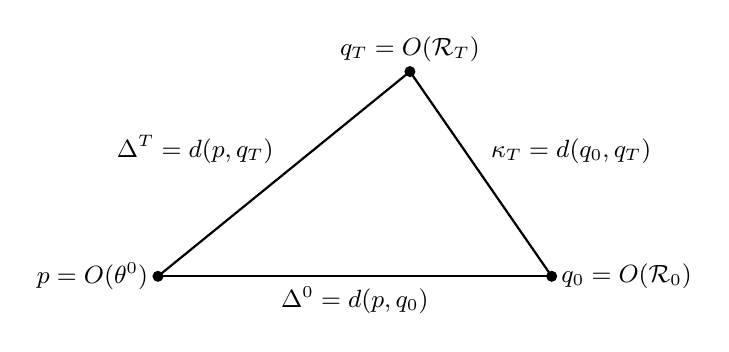
\begin{tikzpicture}[>=stealth, every node/.style={font=\small}]
\coordinate (p) at (0,0);
\coordinate (q0) at (5,0);
\coordinate (qT) at (3.2,2.6);
\draw[thick] (p) -- node[below] {$\Delta^0=d(p,q_0)$} (q0);
\draw[thick] (p) -- node[above left] {$\Delta^T=d(p,q_T)$} (qT);
\draw[thick] (q0) -- node[above right] {$\kappa_T=d(q_0,q_T)$} (qT);
\fill (p) circle (2pt) node[left] {$p=O(\theta^0)$};
\fill (q0) circle (2pt) node[right] {$q_0=O(\mathcal R_0)$};
\fill (qT) circle (2pt) node[above] {$q_T=O(\mathcal R_T)$};
\end{tikzpicture}
\caption{The compensation-gap triangle in observable space. The triangle inequality gives $|\Delta^0-\Delta^T|\le\kappa_T$, which is the content of Lemma~\ref{lem:gap}.}
\end{figure}


The lemma is elementary but it converts a heuristic into a bound. If an acute ablation produces a visible effect and a chronic ablation produces none, the system has demonstrably done something between the two, and the magnitude of what it did is at least the difference. The null is thereby a positive measurement of the system's capacity to reconfigure.

%------------------------------------------------------------------
\section{Four Readings of a Null Ablation}\label{sec:readings}
%------------------------------------------------------------------

The experimental statement
\begin{quote}
\emph{We removed $C$, and nothing happened.}
\end{quote}
can be given four progressively richer interpretations. They are not nested in logical strength. Each is a different claim about the system, and each requires different evidence to be supported and different evidence to be refuted.

\paragraph{First reading: $C$ does nothing.}
The strongest and most naive reading holds that $C$ contributes nothing to the behavior of interest in any regime. Evidence for it would consist of null effects across the full range of operating conditions, at fine resolution, under joint ablations with every plausible partner, and at every adaptation horizon. No ablation study of realistic size provides this. The reading is almost always asserted on the basis of a single condition.

\paragraph{Second reading: $C$ is redundant.}
Here $C$ does contribute, but its contribution is duplicated by another component, so that the system tolerates its loss. This is a claim about the structure of the system at baseline, independent of any adaptive response. It predicts that a joint ablation of $C$ and its duplicate is non-null, and it predicts that the acute effect $\Delta^0$ is already null. It is supported by demonstrating both.

\paragraph{Third reading: another pathway compensated.}
The contribution of $C$ was real and was actively made up by the system. This claim concerns dynamics. It predicts a non-null acute effect $\Delta^0(C)$ that shrinks with horizon $T$, and it predicts a residual in other variables of the system, the trace of the compensating pathway. By Lemma~\ref{lem:gap} it is supported by the pair $(\Delta^0>\varepsilon,\ \Delta^T\le\varepsilon)$.

\paragraph{Fourth reading: the ablation changed the measured system.}
The most general reading holds that the object measured after the intervention is not the original system minus $C$. It is a different system, produced by the intervention together with the system's response. Formally, the experiment measures
\[
\Rop(S,\dox{C=0})\quad\text{and not}\quad S-C .
\]
The third reading is a special case in which the change can be attributed to a specific compensating pathway. The fourth allows that the reconfiguration may be diffuse, nonlocal, or not attributable to any single component, and that the residual state of the whole system, and not merely a scalar output, is what changed.

\begin{table}[h]
\centering
\small
\begin{tabular}{p{2.6cm}p{3.6cm}p{4.3cm}p{3.2cm}}
\toprule
Reading & Claim & Evidence required & Refuted by\\
\midrule
$C$ does nothing & No contribution in any regime & Null across conditions, resolutions, joint ablations, horizons & Any non-null joint or acute effect\\
$C$ is redundant & Contribution duplicated at baseline & Null single, non-null joint with a partner & Non-null single at the same resolution\\
Compensated & System actively re-supplies $C$'s role & Acute effect that decays with $T$; residual in other variables & Flat effect across $T$\\
System changed & Measured object is $\Rop(S,a)$, not $S-C$ & Comparison of $\Rop_0$ and $\Rop_T$; full state readout & Identical full state before and after\\
\bottomrule
\end{tabular}
\caption{Four readings of a null ablation and the evidence that separates them.}
\end{table}

The practical upshot is that a single null observation cannot discriminate among the four. All four predict the same scalar readout at one horizon. The readings separate only when one adds joint ablations, multiple horizons, or richer observables. An ablation study reporting a single null on a single scalar has therefore not yet said which of the four it has found.

%------------------------------------------------------------------
\section{Sources of Silence}\label{sec:silence}
%------------------------------------------------------------------

A null ablation, $\Delta O\approx 0$, can arise in at least six ways. The taxonomy below is not exhaustive but each item has a distinct mechanism and a distinct signature under further experiment.

\subsection{Compensation}

The system contains a feedback or adaptation process that restores the observable after perturbation. Homeostatic regulation is the archetype: a variable is held near a setpoint by adjusting other variables, so that removing one source of the regulated quantity is met by increased output from another. Section~\ref{sec:necessity} gives an exact linear model. In biology, compensatory responses to gene deletion are well documented, including cases in which a knockout mutant shows a milder phenotype than an acute knockdown of the same gene, because the mutation triggers upregulation of related genes~\cite{rossi2015,elbrolosy2019}. In artificial networks, ablating an attention layer in a language model can leave the output almost unchanged because later layers shift their contribution, an effect described as self-repair~\cite{mcgrath2023}.

\subsection{Saturation}

The observable depends on $C$ through a nonlinearity that flattens at the operating point. Let $O=\sigma(c+r)$ with $\sigma=\tanh$, ablated component value $c=1$ against a background $r=5$. Then $O(6)=\tanh 6\approx 0.999988$ and $O(5)=\tanh 5\approx 0.999909$, so $\Delta O\approx 8\times 10^{-5}$, far below any realistic tolerance. Yet at $r=0$ the same ablation moves the output from $\tanh 1\approx 0.762$ to $0$. The component is neither irrelevant nor redundant. It is masked by the regime. Saturating nonlinearities in neural networks, ceiling effects in behavioral measures, and rate-limiting steps in metabolic pathways all produce this pattern.

\subsection{Degeneracy}

The observable factors through a many-to-one map. Write $O=h\circ g$ where $g:\Theta\to G$ has fibres $g^{-1}(y)$ containing many configurations. Edelman and Gally use the term degeneracy for the capacity of structurally different elements to yield the same function~\cite{edelman2001}. If some configuration in the baseline's fibre has $\theta_C=0_C$, then that configuration realizes the same observable without $C$. Degeneracy is a static property of the map, whereas compensation is a dynamic property of the flow. A degenerate system need not adapt at all, provided the ablation happens to land in the fibre. The distinction is examined formally in Section~\ref{sec:necessity}.

\subsection{Measurement coarseness}

The observable is a projection $\pi:Y\to Y'$ of a richer quantity, and the ablation moves the richer quantity without moving the projection. A pass/fail metric, a benchmark accuracy with finite item resolution, a mean over a population in which shifts cancel, and a coarse behavioral score are all projections. If accuracy is computed on $500$ items, no change smaller than $0.2$ percentage points is resolvable in a single evaluation, whatever happens to the underlying log-likelihoods. A statistical version of the same point is that failure to reject a null hypothesis is not evidence for it, a principle summarized in the slogan that absence of evidence is not evidence of absence~\cite{altman1995}, and addressed operationally by equivalence testing~\cite{lakens2017}.

\subsection{Load redistribution}

The system carries a conserved or budgeted quantity, and removing one carrier shifts the burden to the others. A deck supported by $n$ identical parallel members, each of stiffness $k$, under total load $W$, carries $W/n$ per member. Removing one leaves $W/(n-1)$ per survivor, an increase by the factor $n/(n-1)$. If the coarse observable is ``the deck stands'' then the ablation is null provided the survivors have capacity above $W/(n-1)$. The fine observable, strain in the survivors, is not null. It rises by exactly the factor above, and that factor identifies $n$. This example returns in Section~\ref{sec:tomography}. Nothing about it is exotic: the ordinary vocabulary of statically indeterminate structures already treats redundancy as load that can be rerouted.

\subsection{Level-set coincidence}

The finite intervention lands on another point of the same level set of the observable, as in Example~\ref{ex:sin}. Periodic and symmetric systems produce this exactly, and it can occur approximately whenever the response is non-monotone. It is the purely geometric source of silence, requiring neither adaptation nor redundancy.

\begin{table}[h]
\centering
\small
\begin{tabular}{p{2.7cm}p{4.0cm}p{5.4cm}}
\toprule
Source & Mechanism & Distinguishing test\\
\midrule
Compensation & Adaptation restores $O$ & Acute effect present, chronic effect absent; residual in effort variables\\
Saturation & Flat response at the operating point & Vary background; effect returns off saturation\\
Degeneracy & $O=h\circ g$, fibre meets $\theta_C=0$ & Joint ablation with partner is non-null\\
Coarseness & Projection hides change & Finer observable, full state readout\\
Load redistribution & Conserved budget rerouted & Survivor variables shift by predictable factor\\
Level-set coincidence & Finite step lands on same $O$ & Ablate to several nonzero values\\
\bottomrule
\end{tabular}
\caption{Sources of silence and the further experiment that separates each.}
\end{table}

\subsection{Tolerances do not compose}

A further property of the null result deserves its own statement. If each of $n$ single ablations is $\varepsilon$-null, one would like to conclude that ablating all $n$ is at most $n\varepsilon$-null. This holds for additive systems and fails otherwise.

\begin{proposition}[Nulls need not compose]\label{prop:compose}
(i) If $O(\theta)=o_0+\sum_{c}o_c(\theta_c)$ is additive, and each single ablation satisfies $|O(\theta^0)-O(0_c,\theta^0_{-c})|\le\varepsilon$, then ablating any set $D$ changes $O$ by at most $|D|\varepsilon$.
(ii) For every $n\ge 2$ there is a system with $n$ components in which every single ablation is exactly null and the joint ablation of all components has effect $1$.
\end{proposition}
\begin{proof}
(i) Ablating $D$ changes $O$ by $\sum_{c\in D}\bigl(o_c(0_c)-o_c(\theta^0_c)\bigr)$, whose absolute value is at most $\sum_{c\in D}\varepsilon=|D|\varepsilon$. (ii) Let each $\theta_c\in\{0,1\}$, and let $O(\theta)=\max_c\theta_c$ (an OR gate), with baseline $\theta^0=(1,\dots,1)$. Removing one component leaves $n-1\ge 1$ components at $1$, so $O=1$ and the single effect is $0$. Removing all components gives $O=0$, an effect of $1$.
\end{proof}

Part (ii) is the OR gate, the simplest redundancy. It shows that the bound in (i) is a feature of additivity, not of ablation, and that nothing controls the joint effect of a family of null singles unless the system's interaction structure is known.

%------------------------------------------------------------------
%------------------------------------------------------------------
\section{The Geometry of Null Sets}\label{sec:geometry}
%------------------------------------------------------------------

Section~\ref{sec:silence} listed six sources of silence as if they were separate mechanisms. A single geometric statement contains all of them. It concerns the set of configurations that the observable cannot tell apart from the baseline.

\begin{definition}[Null sets]
The \emph{exact null set} (fibre) of $\theta\in\Theta$ is $N(\theta)=O^{-1}\bigl(O(\theta)\bigr)$, and $\theta\sim_O\theta'$ means $O(\theta)=O(\theta')$. The \emph{tolerance set} is $N_\varepsilon(\theta)=\{\theta'\in\Theta:\ d(O(\theta'),O(\theta))\le\varepsilon\}$.
\end{definition}

\begin{remark}[Tolerance is not an equivalence]
The relation $\theta'\in N_\varepsilon(\theta)$ is reflexive and symmetric but not transitive, so $N_\varepsilon(\theta)$ is a neighbourhood and not an equivalence class. Only the exact relation $\sim_O$ partitions $\Theta$. For $O(\theta)=\theta\in\R$ and $\varepsilon=1$, one has $0\in N_1(1)$ and $1\in N_1(2)$, yet $0\notin N_1(2)$. Chains of $\varepsilon$-null steps can therefore accumulate an arbitrarily large effect, which is the geometric form of Proposition~\ref{prop:compose}.
\end{remark}

\begin{proposition}[Null ablation as membership]\label{prop:member}
The ablation $\dox{C=0}$ at horizon $T$ is $\varepsilon$-null if and only if $\Rop_T(S,\dox{C=0})\in N_\varepsilon(\theta^0)$, and exactly null if and only if $\Rop_T(S,\dox{C=0})\in N(\theta^0)$.
\end{proposition}
\begin{proof}
This is Definition of $\Delta^T$ restated: $\Delta^T\le\varepsilon$ means $d(O(\theta^0),O(\Rop_T))\le\varepsilon$.
\end{proof}

The proposition is trivial, and its value is that it recasts each source of silence as a reason why the intervention ends inside the same observational neighbourhood.

\begin{table}[h]
\centering
\small
\begin{tabular}{p{2.8cm}p{9.2cm}}
\toprule
Source & Geometric statement\\
\midrule
Compensation & The adaptation flow steers $\Rop_0$ into $N_\varepsilon(\theta^0)$\\
Degeneracy & $N_\varepsilon(\theta^0)$ meets the ablation slice $\{\theta_C=0_C\}$ (the fibre is nonempty there)\\
Saturation & $\theta^0$ and $\Rop_0$ lie in a region where $DO\approx0$, so $N_\varepsilon(\theta^0)$ contains a neighbourhood\\
Coarseness & A coarser metric $d$ or a many-to-one projection enlarges $N_\varepsilon$\\
Load redistribution & The flow is confined to a conserved slice on which the coarse observable is constant\\
Level-set coincidence & $\Rop_0$ lands on $N(\theta^0)$ without any adaptation\\
\bottomrule
\end{tabular}
\caption{The six sources of silence as statements about $N_\varepsilon(\theta^0)$.}
\end{table}

\begin{figure}[ht]
\centering
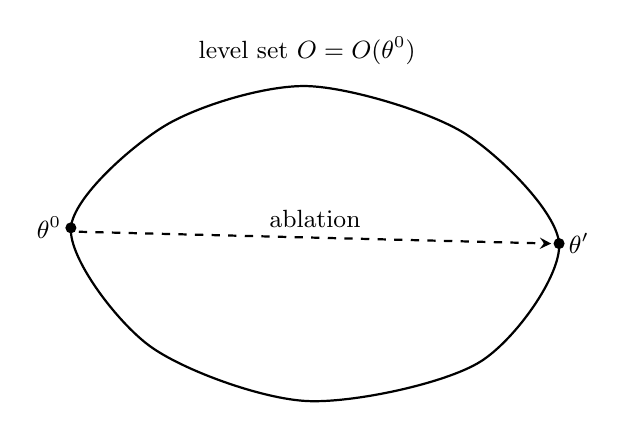
\begin{tikzpicture}[>=stealth, every node/.style={font=\small}]
\draw[thick] plot[smooth cycle] coordinates {(0,2) (2,1.4) (3.2,0) (2.2,-1.5) (0,-2) (-2,-1.3) (-3,0.2) (-1.8,1.5)};
\node at (0,2.45) {level set $O=O(\theta^0)$};
\fill (-3,0.2) circle (2pt) node[left] {$\theta^0$};
\fill (3.2,0) circle (2pt) node[right] {$\theta'$};
\draw[->,thick,dashed] (-2.9,0.15) -- (3.1,0.0) node[midway,above] {ablation};
\end{tikzpicture}
\caption{A null ablation as a move between two points of one level set. The configurations differ, $\theta^0\ne\theta'$, while $O(\theta^0)=O(\theta')$. The path between them need not stay on the level set; only its endpoint is constrained.}
\end{figure}

\subsection{Two geometries of silence}

The table treats every source alike, but two different geometric situations underlie it, and they differ in how likely an exact null is.

Suppose $\Theta$ is a smooth manifold of dimension $D$ and $O:\Theta\to\R^m$ is smooth.

\begin{proposition}[Dimension of exact null sets]\label{prop:dimension}
If $DO(\theta^0)$ has rank $m$ (the point is regular), then near $\theta^0$ the null set $N(\theta^0)$ is an embedded submanifold of dimension $D-m$.
\end{proposition}
\begin{proof}
This is the regular value theorem, a consequence of the implicit function theorem: a submersion has locally a coordinate form $(u_1,\dots,u_D)\mapsto(u_1,\dots,u_m)$, whose level sets are affine subspaces of dimension $D-m$.
\end{proof}

A low-dimensional observable on a high-dimensional configuration space therefore has a high-dimensional null set: room exists to move a very long way without changing $O$. In the homeostat, $D=2$, $m=1$, and the null set is a line (Figure~\ref{fig:homeoplane} below).

A caution is needed. The null set has codimension $m$, hence Lebesgue measure zero in $\Theta$. A passive finite ablation of a non-adaptive system does not land on it except by coincidence. Exact nulls are typical only in two situations.
\begin{enumerate}[label=(\alph*)]
\item \emph{Flat regions.} On an open set where $\operatorname{rank}DO<m$ (saturation, thresholds, dead units), $N(\theta)$ has nonempty interior and a passive step stays inside it with positive probability.
\item \emph{Steering.} The adaptation flow drives the trajectory onto the null set. Regulated systems show exact nulls robustly, and not by accident, because the dynamics are designed or selected to return to the fibre.
\end{enumerate}
Dimension supplies the room for compensation. It does not supply the landing. This distinction separates the passive sources of silence (saturation, coarseness, level-set coincidence) from the active one (compensation).

\subsection{Compensating configurations form a family}

\begin{proposition}[Degeneracy dimension]\label{prop:degdim}
Let $O_0(q)=O(0_C,q)$ for $q\in\Theta_{-C}$, with $\dim\Theta_{-C}=D_{-C}\ge m$. Suppose $O_0$ is a submersion at $q_0=\theta^0_{-C}$. Then there is an open set $U\ni O(\Rop_0)$ in $\R^m$ such that every $y\in U$ is attained: the set $\{q:O_0(q)=y\}$ is nonempty, and near each of its points it is a submanifold of dimension $D_{-C}-m$. In particular, if $O(\theta^0)\in U$, that is, if the static effect $\Delta^0$ is small enough, then compensating configurations exist and form a $(D_{-C}-m)$-parameter family.
\end{proposition}
\begin{proof}
A submersion is locally open, so there is a neighbourhood $W$ of $q_0$ with $U:=O_0(W)$ open, and $O(\Rop_0)=O_0(q_0)\in U$. For $y\in U$ the level set inside $W$ is nonempty and, by the regular value theorem, a submanifold of dimension $D_{-C}-m$.
\end{proof}

The proposition splits the hidden positive content of a null (Corollary~\ref{cor:hidden}) into two parts. That a compensating configuration \emph{exists} is generic when there are more free coordinates than observables and the static effect is small. Which member of the $(D_{-C}-m)$-parameter family the system actually reaches is determined by the adaptation field $V$. The null therefore certifies reachability and not merely existence.

\begin{figure}[ht]
\centering
\begin{tikzpicture}[>=stealth, every node/.style={font=\small}, scale=0.8]
\draw[->] (-0.6,0) -- (5.2,0) node[right] {$x_1$};
\draw[->] (0,-0.6) -- (0,5.2) node[above] {$x_2$};
\draw[thick] (-0.4,4.4) -- (4.4,-0.4);
\node[above right] at (3.0,0.9) {$Y=y^*$};
\fill (2,2) circle (2pt);
\fill (0,4) circle (2pt);
\node[above right] at (2,2) {$\theta^0$};
\node[left] at (0,4) {$\mathcal R_\infty$};
\draw[->,dashed] (2,2) -- (0.1,3.9);
\end{tikzpicture}
\caption{In the homeostat the null set of $Y=x_1+x_2$ is the line $x_1+x_2=y^*$ (dimension $D-m=1$). The chronic ablation moves along it, from $\theta^0$ to $\mathcal R_\infty$.}
\label{fig:homeoplane}
\end{figure}

%------------------------------------------------------------------
\section{Ablation as Quotient Observation}\label{sec:quotient}
%------------------------------------------------------------------

The relation $\sim_O$ is an equivalence relation, so it has a quotient. Let $\pi:\Theta\to\Theta/{\sim_O}$ send a configuration to its class. By the first isomorphism theorem for sets, the quotient is in bijection with the image $O(\Theta)$, and $\pi$ corresponds to $O$ itself. An experiment that records only $O$ does not observe $\Theta$. It observes $\Theta/{\sim_O}$.

\begin{proposition}[Nothing happened in the quotient]\label{prop:quotient}
The ablation trajectory in $\Theta$ is the jump $\theta^0\mapsto\Rop_0$ followed by the flow $t\mapsto\Rop_t$. Its image in observable space is the path $O(\theta^0)\to O(\Rop_0)\to O(\Rop_t)$. The ablation is exactly null at horizon $T$ if and only if this path returns to its starting point, $O(\Rop_T)=O(\theta^0)$. The excursion amplitude
\[
\Xi_T=\sup_{0\le t\le T}d\bigl(O(\theta^0),O(\Rop_t)\bigr)
\]
satisfies $\Xi_T\ge\Delta^0$ and $\Xi_T\ge\Delta^t$ for every $t\le T$, so a null endpoint is compatible with an arbitrarily large excursion.
\end{proposition}
\begin{proof}
The first claim is the definition of exact nullness. The inequalities hold because $t=0$ is included in the supremum and each $\Delta^t$ is one of the distances whose supremum is taken. Arbitrary size follows from Example~\ref{ex:homeostat}: $\Xi_\infty\ge a$ while $\Delta^\infty=0$, with $a$ free.
\end{proof}

In this language, an ablation with nonzero acute effect and zero chronic effect is a closed excursion in the quotient. Its size is the transient the compensation had to overcome, and a study that samples only the endpoint has observed only the point at which the loop closes.

The quotient formulation also says what ``nothing happened'' can mean. It does not mean that the configuration is unchanged. It means that the configuration moved within a fibre of $O$, or left it and returned. A precise statement of the central thesis follows.

\begin{quote}
\textbf{Invariance is not absence of change. It is change constrained to remain invisible under a specified observation map.}
\end{quote}

\begin{figure}[ht]
\centering
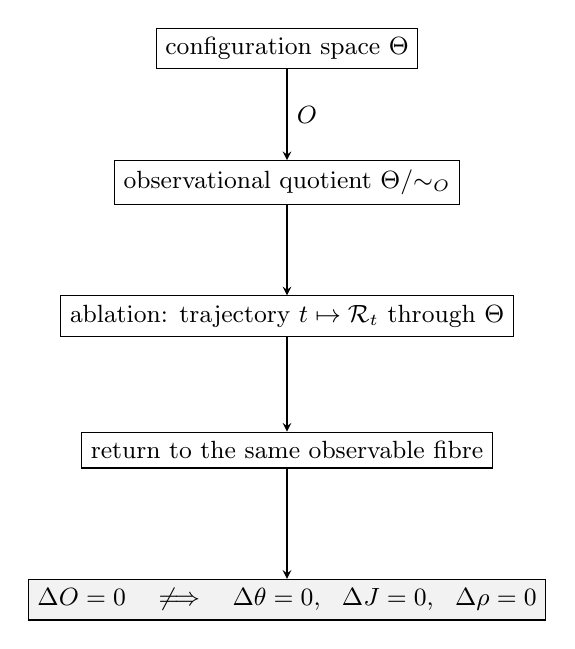
\begin{tikzpicture}[>=stealth, every node/.style={font=\small,align=center}, node distance=1.0cm]
\node[draw,rectangle] (a) at (0,0) {configuration space $\Theta$};
\node[draw,rectangle] (b) at (0,-1.7) {observational quotient $\Theta/{\sim_O}$};
\node[draw,rectangle] (c) at (0,-3.4) {ablation: trajectory $t\mapsto\mathcal R_t$ through $\Theta$};
\node[draw,rectangle] (d) at (0,-5.1) {return to the same observable fibre};
\node[draw,rectangle,fill=gray!10] (e) at (0,-7.0) {$\Delta O=0\quad\not\Longrightarrow\quad\Delta\theta=0,\ \ \Delta J=0,\ \ \Delta\rho=0$};
\draw[->] (a) -- node[right] {$O$} (b);
\draw[->] (b) -- (c);
\draw[->] (c) -- (d);
\draw[->] (d) -- (e);
\end{tikzpicture}
\caption{The observational spine. Here $J$ is the compensation cost of Section~\ref{sec:cost} and $\rho$ the robustness margin of Section~\ref{sec:slack}.}
\end{figure}

The two extra quantities in the last box are developed in Sections~\ref{sec:cost} and~\ref{sec:slack}. Output invariance can coexist with a change of configuration, with a cost incurred to maintain the output, and with a loss of margin against failure. Each is a distinction erased by $O$ and recoverable only by a different observer, a point taken up formally in Section~\ref{sec:observer}.

%------------------------------------------------------------------
\section{Component Necessity and Path Necessity}\label{sec:necessity}
%------------------------------------------------------------------

\subsection{Structure functions, paths, and cuts}

To separate what a component does from what a single ablation reveals, it helps to borrow the language of coherent systems from reliability theory~\cite{barlow1975}. For $z\in\{0,1\}^K$, let $O(z)$ denote the observable when the components with $z_c=1$ are retained and the others ablated, and write $\mathbf 1$ for the all-retained vector. Identify $z$ with the retained set $\{c:z_c=1\}$. Assume $O$ is real-valued and \emph{monotone}: retaining more components never lowers $O$.

\begin{definition}[Paths and cuts]
A set $P\subseteq K$ is an \emph{$\varepsilon$-path} if retaining exactly $P$ leaves $O$ within $\varepsilon$ of the full system: $|O(\mathbf 1)-O(\mathbf 1_P)|\le\varepsilon$. A set $D\subseteq K$ is an \emph{$\varepsilon$-cut} if ablating $D$ moves $O$ by more than $\varepsilon$: $|O(\mathbf 1)-O(\mathbf 1_{K\setminus D})|>\varepsilon$. A minimal path (cut) is one with no proper subset that is a path (cut).
\end{definition}

For monotone $O$ the two notions are complementary: $D$ is a cut exactly when $K\setminus D$ is not a path. A component $c$ is \emph{necessary} if $\{c\}$ is a cut. It is \emph{used} if it belongs to at least one minimal path. Necessity and use come apart.

\begin{proposition}[Necessity is membership in the core]\label{prop:core}
For monotone $O$, component $c$ is necessary if and only if $c$ lies in every $\varepsilon$-path. Equivalently, the set of necessary components is the intersection $\bigcap\{P:P\text{ an }\varepsilon\text{-path}\}$, which is called the \emph{core}.
\end{proposition}
\begin{proof}
Suppose $c$ is necessary, so $K\setminus\{c\}$ is not a path. If some path $P$ avoided $c$, then $P\subseteq K\setminus\{c\}$ and by monotonicity $O(\mathbf 1_P)\le O(\mathbf 1_{K\setminus c})\le O(\mathbf 1)$, so $|O(\mathbf 1)-O(\mathbf 1_{K\setminus c})|\le|O(\mathbf 1)-O(\mathbf 1_P)|\le\varepsilon$, contradicting that $K\setminus c$ is not a path. Hence every path contains $c$. Conversely, if every path contains $c$ then $K\setminus\{c\}$ is not a path, so $\{c\}$ is a cut.
\end{proof}

The consequence is that a single-ablation study measures exactly membership in the core, and nothing else about the path structure. The core may be empty in a system in which every component is used.

\begin{example}[Threshold systems]
Let $O(z)=\ind\bigl[\sum_c z_c\ge r\bigr]$ with $1\le r<n$. Every set of size at least $r$ is a path, so every $r$-subset is a minimal path and every component is used. The core is empty for $r<n$, so every single ablation is null. Component necessity is zero across the board while the system is entirely built from these components. Minimal cuts have size $n-r+1$, and that number, not any single-ablation statistic, is the redundancy of the system.
\end{example}


\begin{figure}[ht]
\centering
\begin{minipage}{0.44\textwidth}
\centering
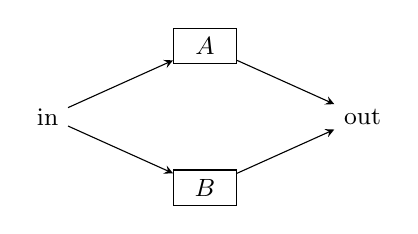
\begin{tikzpicture}[>=stealth, every node/.style={font=\small}]
\node (in) at (0,0) {in};
\node (out) at (4,0) {out};
\node[draw,rectangle,minimum width=0.8cm] (A) at (2,0.9) {$A$};
\node[draw,rectangle,minimum width=0.8cm] (B) at (2,-0.9) {$B$};
\draw[->] (in) -- (A);
\draw[->] (A) -- (out);
\draw[->] (in) -- (B);
\draw[->] (B) -- (out);
\end{tikzpicture}
\end{minipage}\hfill
\begin{minipage}{0.52\textwidth}
\small
\begin{tabular}{ll}
remove $A$: & path $B$ survives\\
remove $B$: & path $A$ survives\\
remove $A,B$: & \textbf{cut}\\[4pt]
minimal paths: & $\{A\},\ \{B\}$\\
core: & $\{A\}\cap\{B\}=\emptyset$
\end{tabular}
\end{minipage}
\caption{Two parallel routes. Both components are used, neither is necessary, and the core is empty. Every single ablation is null; the joint ablation is not.}
\end{figure}

\subsection{Degeneracy as invariance}

The static source of silence identified in Section~\ref{sec:silence} can be stated exactly.

\begin{proposition}[Fibre invariance]\label{prop:fibre}
Suppose $O=h\circ g$ with $g:\Theta\to G$. Let $\theta^0$ be the baseline and suppose the reconfiguration operator selects a configuration in the fibre:
\[
\Rop_T(S,\dox{C=0})\in g^{-1}\bigl(g(\theta^0)\bigr)\cap\{\theta_C=0_C\}.
\]
Then $\Delta^T(C)=0$ exactly, for any $h$.
\end{proposition}
\begin{proof}
$O(\Rop_T)=h(g(\Rop_T))=h(g(\theta^0))=O(\theta^0)$.
\end{proof}

The hypothesis has two parts, and they correspond to two different claims. That the fibre $g^{-1}(g(\theta^0))\cap\{\theta_C=0_C\}$ is nonempty is a claim about degeneracy: there \emph{exists} a $C$-free configuration with the same observable. That the operator \emph{selects} such a configuration is a claim about dynamics: the system can \emph{reach} it. A null ablation certifies both at once, which is the hidden positive content of the null.

\begin{corollary}[The null contains a positive result]\label{cor:hidden}
If $\Delta^T(C)=0$ then there exists a configuration $\theta'$ with $\theta'_C=0_C$, $O(\theta')=O(\theta^0)$, and $\theta'$ reachable from $\theta^0$ under the adaptation flow with $C$ pinned. In the notation of the compensated form
\[
f(0,P_2',\dots,P_n')\approx f(P_1,P_2,\dots,P_n),\qquad P_j\longrightarrow P_j'\ (j\ge 2),
\]
the map $P_{-1}\mapsto P_{-1}'$ is a \emph{compensatory transformation} realized by the system itself.
\end{corollary}

In words: a null ablation of component $1$ shows that the remaining components possess a transformation which restores the function. The existence of that transformation is a fact about the system that a non-null ablation would not have revealed.

\subsection{An exact model of compensation}

The following linear model isolates the distinction between the static sensitivity of a variable and its sensitivity at equilibrium.

\begin{example}[Homeostat with two sources]\label{ex:homeostat}
Let $Y=x_1+x_2$ be a regulated quantity with setpoint $y^*$. The source $x_1$ is the ablation target. The second source $x_2$ is adjusted by a controller with gain $k>0$:
\[
\dot x_2=-k\,(x_1+x_2-y^*).
\]
For fixed $x_1$ the unique rest point is $x_2^*=y^*-x_1$, and it is globally asymptotically stable because the equation is a stable linear relaxation. At baseline $x_1=a$ and $x_2^*=y^*-a$, so $Y=y^*$.

\emph{Static sensitivity.} With $x_2$ held fixed, $\partial Y/\partial x_1=1$. Ablating $x_1$ from $a$ to $0$ gives the static effect $\Delta^0=a$.

\emph{Chronic sensitivity.} Letting $x_2$ relax, $Y^*=y^*$ for every value of $x_1$, so $\partial Y^*/\partial x_1=0$ and $\Delta^\infty=0$.

\emph{Residual.} The shift in the effort variable is $x_2^*(0)-x_2^*(a)=a$. It equals exactly the amount removed.
\end{example}

Three observations follow. First, the observable $Y$ is null after ablation while its static sensitivity is $1$, the maximal value for this model, so the implication \eqref{eq:central} fails in the strongest possible way. Second, the compensation gap is $\kappa_\infty=a$, so by Lemma~\ref{lem:gap} the null result is a measurement of the amount compensated. Third, the information the experiment discarded lies in $x_2$, not in $Y$. The general principle is worth naming.

\begin{proposition}[Regulated and effort variables]\label{prop:effort}
Suppose a regulated variable $g(\theta)$ is held at $y^*$ by adaptation of free coordinates, in the sense that for every admissible pinned value of $\theta_C$ the free dynamics have an asymptotically stable set contained in $\{g=y^*\}$ that attracts the trajectory from $\theta^0_{-C}$. Then the chronic effect of any ablation of $C$ on $g$ is zero, and any information about $C$'s contribution is carried by the free (effort) coordinates.
\end{proposition}
\begin{proof}
By hypothesis $\lim_{T\to\infty}g(\Rop_T)=y^*=g(\theta^0)$, so $\Delta^\infty=0$ for the observable $g$. Since the pinned coordinate values differ between baseline and ablated system while $g$ is equal, the difference in $C$'s role must be absorbed by $\theta_{-C}$: if $\theta_{-C}$ also coincided, the two configurations would be identical, contradicting $\theta_C\ne 0_C$ at baseline.
\end{proof}

The proposition explains a pattern that recurs across fields. Homeostatic quantities such as blood glucose, body temperature, and the output of a well-tuned network appear robust to removal of individual contributors, and the contributors' identities are found instead in the effort variables: hormone levels, metabolic flux, weights redistributed across layers. Studies that record only the regulated quantity see a null. Studies that record the effort variables see the compensation.

\begin{figure}[h]
\centering
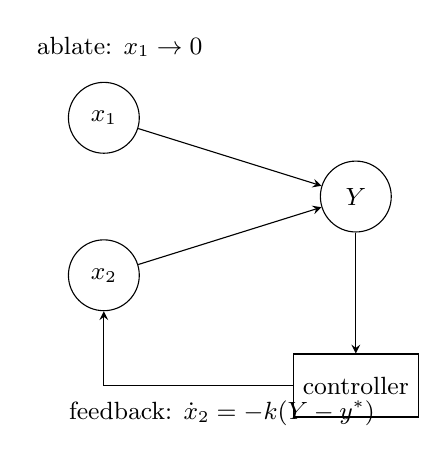
\begin{tikzpicture}[>=stealth, every node/.style={font=\small}]
\node[draw,circle,minimum size=0.9cm] (x1) at (0,1) {$x_1$};
\node[draw,circle,minimum size=0.9cm] (x2) at (0,-1) {$x_2$};
\node[draw,circle,minimum size=0.9cm] (Y) at (3.2,0) {$Y$};
\node[draw,rectangle,minimum height=0.8cm] (ctl) at (3.2,-2.4) {controller};
\draw[->] (x1) -- (Y);
\draw[->] (x2) -- (Y);
\draw[->] (Y) -- (ctl);
\draw[->] (ctl) -| (x2);
\node at (0.2,1.9) {ablate: $x_1\to 0$};
\node at (1.5,-2.75) {feedback: $\dot x_2=-k(Y-y^*)$};
\end{tikzpicture}
\caption{Ablating $x_1$ leaves the regulated quantity $Y$ unchanged, because the controller raises $x_2$ by exactly the amount removed.}
\end{figure}

\subsection{The subtraction fallacy}

The pieces assemble into the main structural claim.

\begin{theorem}[Ablation is not subtraction]\label{thm:notsub}
In general
\[
S-C\ \neq\ \Rop(S,\dox{C=0}).
\]
More precisely, for any adaptive system with nonzero adaptation on the free coordinates, $\Rop_T(S,\dox{C=0})\ne\Rop_0(S,\dox{C=0})$ for all $T>0$ at which the free trajectory has moved. The compensation gap $\kappa_T(C)$ may be arbitrarily large while $\Delta^T(C)=0$.
\end{theorem}
\begin{proof}
The static ablation $\Rop_0$ is the subtraction $S-C$ by definition. The configuration $\Rop_T$ differs from it precisely by the displacement $\psi^a_T(\theta^0_{-C})-\theta^0_{-C}$ of the free coordinates, which is nonzero whenever the trajectory has left its initial point. For the second claim, Example~\ref{ex:homeostat} gives $\Delta^\infty=0$ and $\kappa_\infty=a$ with $a$ arbitrary.
\end{proof}

The theorem gives a precise meaning to the claim that an ablation experiment is ordinarily narrated as subtraction but is actually a perturbation followed by reconstruction. In what follows $\Rop(S,\dox{C=0})$ is the experimental object, and $S-C$ is a counterfactual that may not be realized by any experiment on an adaptive system.


\begin{figure}[ht]
\centering
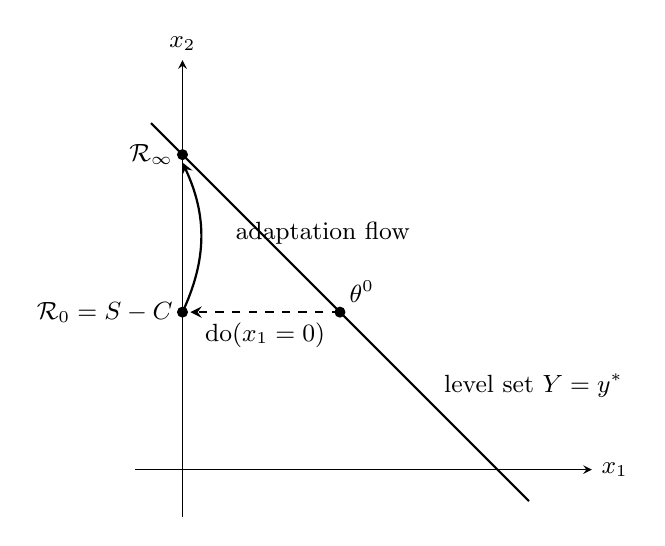
\begin{tikzpicture}[>=stealth, every node/.style={font=\small}]
\draw[->] (-0.6,0) -- (5.2,0) node[right] {$x_1$};
\draw[->] (0,-0.6) -- (0,5.2) node[above] {$x_2$};
\draw[thick] (-0.4,4.4) -- (4.4,-0.4);
\node[above right] at (3.2,0.8) {level set $Y=y^*$};
\fill (2,2) circle (2pt) node[above right] {$\theta^0$};
\fill (0,2) circle (2pt) node[left] {$\mathcal R_0=S-C$};
\fill (0,4) circle (2pt) node[left] {$\mathcal R_\infty$};
\draw[->,thick,dashed] (2,2) -- (0.1,2) node[midway,below] {$\mathrm{do}(x_1=0)$};
\draw[->,thick] (0,2) to[bend right=25] (0,3.9);
\node[right] at (0.55,3.0) {adaptation flow};
\end{tikzpicture}
\caption{The homeostat of Example~\ref{ex:homeostat} in configuration space, with $a=2$ and $y^*=4$. Subtraction moves the configuration off the regulated level set to $S-C$. The adaptation flow carries it back onto the level set at a different point, a displacement of $a$ in the effort coordinate $x_2$. The observable is unchanged; the configuration is not.}
\end{figure}

The two cases of the theorem, static and dynamic, admit a two-by-two classification by whether the static and reconfigured effects are null.

\begin{table}[h]
\centering
\small
\begin{tabular}{p{3.2cm}p{4.0cm}p{5.2cm}}
\toprule
 & $\Delta^T\le\varepsilon$ & $\Delta^T>\varepsilon$\\
\midrule
$\Delta^0\le\varepsilon$ & Inert at this operating point (or masked by saturation, coarseness, level-set coincidence) & Destabilization: the reconfiguration itself is harmful\\
$\Delta^0>\varepsilon$ & Compensated: $\kappa_T\ge\Delta^0-\varepsilon$ & Necessary on the tested horizon\\
\bottomrule
\end{tabular}
\caption{Classification by static and reconfigured effect. Only the lower left cell licenses the statement that the system compensated.}
\label{tab:class}
\end{table}

Most published ablation studies populate only one column and one horizon, and therefore cannot place their component in a cell. That a null study reports a single number is a limitation on what it can say, not on what the system did.


%------------------------------------------------------------------
\section{Timescales: The Horizon Spectrum}\label{sec:time}
%------------------------------------------------------------------

Definition~\ref{def:recon} indexes the reconfiguration operator by a horizon $T$, yet the argument so far has mostly compared the two endpoints $T=0$ and $T=\infty$. Real experiments sit at intermediate horizons that are seldom reported, and the choice of horizon amounts to a choice among different experimental questions. Let $\tau$ denote the characteristic time of the system's adaptation. Three regimes can be distinguished.

\begin{table}[h]
\centering
\small
\begin{tabular}{p{2.0cm}p{2.2cm}p{5.6cm}p{2.2cm}}
\toprule
Regime & Horizon & Typical experiment & Estimates\\
\midrule
Acute & $T\ll\tau$ & Clamp for one forward pass; acute inhibitor; activation patch at inference & $\Delta^0$\\
Transient & $T\sim\tau$ & Short retraining after pruning; hours after a conditional knockout & The trajectory\\
Chronic & $T\gg\tau$ & Germline knockout; retraining to convergence; long-term removal of an office or member & $\Delta^\infty$\\
\bottomrule
\end{tabular}
\caption{Adaptation regimes and the experiments that occupy them.}
\end{table}

The relevant $\tau$ can span several orders of magnitude within a single system. In an organism the adaptation may be physiological (seconds to hours), transcriptional (hours to days), or developmental and evolutionary (generations). In a trained network it may be a single forward pass, a few gradient steps, or a full retraining. The experimental sentence ``we removed $C$'' is silent on which of these applies.

\subsection{The horizon curve of the homeostat}

The exact model of Example~\ref{ex:homeostat} can be solved at every horizon.

\begin{proposition}[Horizon curve]\label{prop:horizon}
In Example~\ref{ex:homeostat}, with baseline contribution $x_1=a>0$ and controller gain $k>0$, the reconfigured effect and compensation gap at horizon $T$ are
\[
\Delta^T=a\,e^{-kT},\qquad \kappa_T=a\bigl(1-e^{-kT}\bigr).
\]
\end{proposition}
\begin{proof}
After ablation $x_1=0$ and $\dot x_2=-k(x_2-y^*)$ with $x_2(0)=y^*-a$. The solution is $x_2(t)=y^*-a\,e^{-kt}$, and $Y=x_2$, so $Y(T)-y^*=-a\,e^{-kT}$ and $\Delta^T=a\,e^{-kT}$. The static ablation has $Y=y^*-a$, so $\kappa_T=|Y(T)-(y^*-a)|=a(1-e^{-kT})$.
\end{proof}

Two consequences follow, and both convert an apparently uninformative null into a measurement.

\begin{corollary}[A null bounds the adaptation rate]\label{cor:rate}
If the static effect $a$ is known and an experiment at horizon $T$ finds $\Delta^T\le\varepsilon$ with $\varepsilon<a$, then
\[
k\ \ge\ \frac1T\ln\frac{a}{\varepsilon}.
\]
\end{corollary}
\begin{proof}
$a e^{-kT}\le\varepsilon$ is equivalent to $e^{-kT}\le\varepsilon/a$, i.e., $kT\ge\ln(a/\varepsilon)$.
\end{proof}

\begin{corollary}[Disagreement without error]\label{cor:disagree}
Let $\tau_\varepsilon=\frac1k\ln\frac a\varepsilon$ be the crossover horizon. Two laboratories ablating the same component in the same system, one at $T_A<\tau_\varepsilon$ and one at $T_B\ge\tau_\varepsilon$, obtain $\Delta^{T_A}>\varepsilon$ and $\Delta^{T_B}\le\varepsilon$. Both are correct.
\end{corollary}
\begin{proof}
$\Delta^T=ae^{-kT}$ is strictly decreasing in $T$ and equals $\varepsilon$ at $T=\tau_\varepsilon$.
\end{proof}

The second corollary describes a familiar situation. A component is reported essential in one study and dispensable in another, and the difference is attributed to error, strain, or context. When the two studies occupy different adaptation regimes, no error is required. The disagreement is a measurement of $\tau_\varepsilon$.

\subsection{Beyond a single time constant}

\begin{remark}[Several modes]
For linear adaptation $\dot x=-M(x-x^*)$ with $M$ having eigenvalues of positive real part $\lambda_1,\dots,\lambda_m$, the effect takes the form $\Delta^T=\bigl|\sum_j c_j e^{-\lambda_jT}\bigr|$ for coefficients $c_j$ determined by the ablation. A single-horizon measurement collapses this spectrum into one number. Separating modes requires recording at several horizons, and recovering rates from a sum of exponentials is numerically ill-conditioned, so the horizons should be spread over more than one decade when the modes are not known in advance.
\end{remark}

\begin{remark}[Zero crossings in time]
When the regulator is second order and underdamped, the deviation of the regulated variable after ablation is not monotone. With natural frequency $\omega$, damping ratio $\zeta<1$, and damped frequency $\omega_d=\omega\sqrt{1-\zeta^2}$, an initial deviation $a$ with zero initial velocity evolves as
\[
e(t)=a\,e^{-\zeta\omega t}\Bigl(\cos\omega_d t+\frac{\zeta\omega}{\omega_d}\sin\omega_d t\Bigr).
\]
This vanishes at the infinitely many times satisfying $\tan(\omega_d t)=-\omega_d/(\zeta\omega)$. An experiment sampling at such a time records $\Delta^T=0$ although the system is mid-transient and will deviate again. This is the temporal counterpart of the level-set coincidence of Example~\ref{ex:sin}, and it is guarded against in the same way, by sampling at several horizons.
\end{remark}

%------------------------------------------------------------------
%------------------------------------------------------------------
\section{The Cost of Invariance}\label{sec:cost}
%------------------------------------------------------------------

Output invariance and cost invariance are different properties. A system can keep $O$ fixed by spending something: energy, bandwidth, latency, capacity, flexibility, or attention. The effort variables of Proposition~\ref{prop:effort} are where the spending appears, and a cost functional turns it into a number.

\begin{definition}[Compensation cost]
Let $c:\Theta\to[0,\infty)$ be a cost rate, with $c(\theta^0)=0$, measuring the excess expenditure relative to baseline. Along the ablated trajectory $\theta(t)=\Rop_t(S,a)$ the accumulated compensation cost is
\[
J_C(T)=\int_0^T c\bigl(\theta(t)\bigr)\,dt .
\]
The choice of $c$ is a modelling decision fixed by what is scarce in the system at hand.
\end{definition}

\begin{proposition}[Invariance without cost invariance]\label{prop:cost}
In Example~\ref{ex:homeostat} take $c(x)=(x_2-x_2^0)^2$. Then $\Delta^\infty=0$, yet
\[
J_C(T)=a^2\Bigl[T-\frac2k\bigl(1-e^{-kT}\bigr)+\frac1{2k}\bigl(1-e^{-2kT}\bigr)\Bigr],
\]
so the cost rate tends to $a^2>0$ and $J_C(T)\sim a^2T$ grows without bound.
\end{proposition}
\begin{proof}
By Proposition~\ref{prop:horizon}, $x_2(t)-x_2^0=a(1-e^{-kt})$, so $c=a^2(1-e^{-kt})^2=a^2(1-2e^{-kt}+e^{-2kt})$. Integrating from $0$ to $T$ gives the stated expression. As $t\to\infty$ the integrand tends to $a^2$.
\end{proof}

The output returned to its baseline, and the system pays a permanent cost to keep it there. Reports that state only $\Delta^T=0$ conceal a running expenditure. The correct summary of the experiment is the pair $\bigl(\Delta^T(C),J_C(T)\bigr)$. The two need not be combined into a scalar. Where a scalar is wanted, two normalizations are defined when $\Delta^0>0$: the fraction restored, $1-\Delta^T/\Delta^0$, and the cost per unit restored, $J_C(T)/(\Delta^0-\Delta^T)$. Neither is defined when $\Delta^0=0$, which is one reason to report the pair.

\subsection{Compensation forces cost}

The cost is not arbitrary. Under mild regularity, any compensation at all incurs a cost that grows with its size.

\begin{proposition}[Compensation forces cost]\label{prop:forced}
Suppose $O$ is $L$-Lipschitz in the free coordinates, $d\bigl(O(0_C,q),O(0_C,q')\bigr)\le L\|q-q'\|$, and the cost is coercive, $c(\theta)\ge\lambda\|\theta_{-C}-\theta^0_{-C}\|^2$ for some $\lambda>0$. Then at every horizon,
\[
c\bigl(\Rop_T(S,a)\bigr)\ \ge\ \lambda\,\frac{\kappa_T(C)^2}{L^2}.
\]
\end{proposition}
\begin{proof}
$\Rop_0$ and $\Rop_T$ share $\theta_C=0_C$ and differ in the free coordinates, which are $\theta^0_{-C}$ and $\psi^a_T(\theta^0_{-C})$. So $\kappa_T=d(O(\Rop_0),O(\Rop_T))\le L\|\psi^a_T(\theta^0_{-C})-\theta^0_{-C}\|$. Hence the displacement is at least $\kappa_T/L$, and coercivity gives the bound.
\end{proof}

The result links the two hidden positive quantities of the essay. The compensation gap $\kappa_T$, which measures how much the system did, lower-bounds the instantaneous cost of doing it. A null with a large gap is an expensive null.

\begin{remark}[Cost is not rebound]
The rebound of Section~\ref{sec:restore} reads the compensation gap in the observable at the instant of restoration, and the cost reads the effort spent in the free coordinates during the ablation. They are different measurements of the same reconfiguration, and they can be compared: in the homeostat the rebound equals $\kappa_T$ while the cost rate at horizon $T$ equals $\kappa_T^2$.
\end{remark}

%------------------------------------------------------------------
\section{Joint Ablations and the Interaction Signature}\label{sec:joint}
%------------------------------------------------------------------

\subsection{The interaction term}

Single ablations are blind to interaction. Let $v(T)=O(\mathbf 1_T)$ be the value with only the set $T$ retained, and write $\Delta_D=v(K)-v(K\setminus D)$ for the effect of ablating $D$. For two components define the interaction
\begin{equation}\label{eq:interaction}
\varepsilon_{CD}=\Delta_{\{C,D\}}-\Delta_{C}-\Delta_{D}.
\end{equation}
When $\varepsilon_{CD}=0$ the two effects add. When it is nonzero, the effect of removing both differs from the sum of the effects of removing each.

\begin{proposition}[Diagnostic signature of compensation]\label{prop:signature}
If $\Delta_C=\Delta_D=0$ and $\Delta_{\{C,D\}}\ne 0$ then $\varepsilon_{CD}=\Delta_{\{C,D\}}\ne 0$, so the system is non-additive on $\{C,D\}$. Conversely, if the system is additive on a set $D_1,\dots,D_m$ and all singles are null, every joint ablation among them is null.
\end{proposition}
\begin{proof}
Substituting the hypotheses into \eqref{eq:interaction} gives the first claim. The converse is Proposition~\ref{prop:compose}(i) with $\varepsilon=0$.
\end{proof}

In genetics this pattern is called synthetic lethality: two single deletions are each viable, and the double deletion is not. The concept has a history extending from early observations of Bridges and Dobzhansky, and it has been used systematically as a tool for finding pairs of genes that compensate for one another~\cite{hartwell1997}. In the terms of this essay, synthetic lethality is the interaction signature of the second and third readings. A null on $C$ alone together with a large effect on $\{C,D\}$ is positive evidence of a compensatory path through $D$.

\subsection{Why single ablations misattribute importance}

The failure extends beyond the binary decision that a component is unimportant. Any importance score computed from single ablations alone misattributes credit in the presence of redundancy. The Shapley value~\cite{shapley1953}, which averages a component's marginal contribution over all orders of retention, gives a contrasting view.

\begin{definition}
For a value function $v$ on subsets of $K$ the Shapley value of $c$ is
\[
\phi_c=\sum_{T\subseteq K\setminus\{c\}}\frac{|T|!\,(n-|T|-1)!}{n!}\bigl[v(T\cup\{c\})-v(T)\bigr].
\]
\end{definition}

\begin{proposition}[Symmetric threshold systems]\label{prop:shapley}
For the $r$-out-of-$n$ threshold system with $1\le r<n$ and $v(T)=\ind[|T|\ge r]$, every single ablation is null, yet $\phi_c=1/n$ for every $c$.
\end{proposition}
\begin{proof}
The single-ablation effect is $v(K)-v(K\setminus c)=1-\ind[n-1\ge r]=0$. All components are exchangeable, so $\phi_c$ is the same for all $c$. By efficiency, $\sum_c\phi_c=v(K)-v(\emptyset)=1-0=1$, hence $\phi_c=1/n$.
\end{proof}

For $n=2$, $r=1$ this is the two-path system of the earlier examples: single ablations are zero and each component receives credit $1/2$. The Shapley value is not offered as the correct notion of importance. The point is that a measure sensitive to the full lattice of retained sets sees what the single-ablation score misses, and that the two disagree exactly when redundancy is present.

\subsection{Order of the required ablation}

If the minimal cuts of a system have size $s$, then no set of ablations of size less than $s$ can detect any effect, and the system will present as fully robust to any study restricted to smaller sets. Redundancy of order $s$ is invisible to all ablations of order $s-1$ or fewer. This is a sharp statement, and it turns the vague worry that a study ``did not test enough'' into a quantitative one.

\begin{proposition}[Invisibility below the cut size]\label{prop:below}
In the $r$-out-of-$n$ threshold system, every ablation of at most $n-r$ components is null, and ablations of $n-r+1$ or more components are non-null.
\end{proposition}
\begin{proof}
Ablating $m$ components retains $n-m$, and the system functions iff $n-m\ge r$, i.e., $m\le n-r$.
\end{proof}


%------------------------------------------------------------------
\section{Ablation Profiles, Margins, and the Sampling Failure of Random Ablation}\label{sec:profile}
%------------------------------------------------------------------

Section~\ref{sec:joint} compared single and paired ablations. This section considers the whole family of ablations of every size, which yields the operational meaning of redundancy.

\subsection{Profiles}

\begin{definition}[Ablation profiles]
For a monotone system, let $D$ be a uniformly random $m$-subset of $K$. The \emph{cut profile} is $A(m)=\Pr[D\text{ is an }\varepsilon\text{-cut}]$, and the \emph{effect profile} is $E(m)=\mathbb E\,|O(\mathbf 1)-O(\mathbf 1_{K\setminus D})|$. Let $s$ be the size of a smallest $\varepsilon$-cut (the \emph{cut number}).
\end{definition}

\begin{proposition}[Monotone profile and margin]\label{prop:margin}
For a monotone system, $A(m)\le A(m+1)$ for all $m$, and $A(m)=0$ if and only if $m<s$. The \emph{tolerance margin} $m^*=s-1$ is therefore the largest number of components that can be removed in any way without exceeding $\varepsilon$.
\end{proposition}
\begin{proof}
Draw a uniformly random $(m+1)$-subset $D'$ and delete one of its elements uniformly at random, producing a uniformly random $m$-subset $D\subseteq D'$. If $D$ is a cut then so is $D'$, because ablating more components cannot bring $O$ closer to its baseline in a monotone system. Hence $A(m+1)\ge A(m)$. If $m\ge s$, a fixed minimal cut of size $s$ is contained in some $m$-subset, so $A(m)>0$; if $m<s$ no $m$-subset is a cut, so $A(m)=0$.
\end{proof}

The margin is the quantity that a single-ablation study cannot see. A study finding every single ablation null has established $m^*\ge1$, which is compatible with $m^*=1$ (a system one removal from failure) and with $m^*=n-1$ (a system with enormous reserve).

\subsection{Shape distinguishes additivity from redundancy}

\begin{proposition}[Flat-then-rise is non-additive]\label{prop:flat}
If $O$ is additive, $O(\theta)=o_0+\sum_c o_c(\theta_c)$, and $E(1)=0$ exactly, then $E(m)=0$ for all $m$. Consequently any system with $E(1)=0$ and $E(m)>0$ for some $m$ is not additive.
\end{proposition}
\begin{proof}
$E(1)=0$ forces every single effect $|o_c(0_c)-o_c(\theta^0_c)|$ to vanish, since $E(1)$ is an average of nonnegative terms. For additive $O$ the effect of any $D$ is the sum of these vanishing terms, hence zero.
\end{proof}

For the threshold system the profile is a step: $E(m)=0$ for $m\le n-r$ and $E(m)=1$ for $m>n-r$. For an additive system with equal contributions $\delta$ it is the line $E(m)=m\delta$. The two shapes are opposite in curvature, and the curvature is itself a coarse measurement of interaction. A profile that is flat and then rises steeply is the signature of a reserve consumed, and the position of the rise is the cut number $s$.

\subsection{Nulls consume margin}

\begin{proposition}[Sequential nulls]\label{prop:consume}
In an $r$-out-of-$n$ threshold system, suppose $j\le n-r$ distinct components have already been ablated. Then every further single ablation is null if $j<n-r$, and the next ablation is fatal if $j=n-r$. The tolerance margin of the surviving system is $n-r-j$.
\end{proposition}
\begin{proof}
After $j$ ablations, $n-j$ components remain, and the system is a threshold system with the same $r$. A further single ablation leaves $n-j-1\ge r$ components exactly when $j<n-r$.
\end{proof}

The proposition has a methodological consequence. If successive ablations are performed on the same specimen, the $j$th null is a statement about a system with reduced margin, and the order of testing matters. Independent specimens (or restoration between ablations, Section~\ref{sec:restore}) are needed to keep each test a test of the intact system. A study that removes components one by one and reports that the system survived each removal has reported a sequence in which the last null may sit one step from a cliff.

\subsection{Why random ablation misses small cuts}

Studies often ablate random subsets, either for convenience or to summarize robustness. A small unique cut can then be missed with high probability.

\begin{proposition}[Random ablation and a unique small cut]\label{prop:random}
Suppose $\varepsilon$-cuts are exactly the sets containing a fixed $s$-subset $S_0$. A uniformly random $m$-subset of $K$ is a cut with probability
\[
\Pr=\frac{\binom{n-s}{m-s}}{\binom nm}=\prod_{i=0}^{s-1}\frac{m-i}{n-i}.
\]
For $s=2$ this equals $\frac{m(m-1)}{n(n-1)}$.
\end{proposition}
\begin{proof}
An $m$-subset contains $S_0$ iff it is $S_0$ together with $m-s$ of the remaining $n-s$ components, which gives the first expression. The product form follows from $\binom{n-s}{m-s}/\binom nm=\frac{m!\,(n-s)!}{n!\,(m-s)!}=\prod_{i=0}^{s-1}\frac{m-i}{n-i}$.
\end{proof}

With $n=1000$ components, $s=2$, and random ablations of size $m=30$, the probability that a trial contains the critical pair is $\frac{30\cdot29}{1000\cdot999}\approx 8.7\times10^{-4}$. About $1150$ random trials are needed to expect a single hit. A random-ablation curve for this system would show smooth robustness up to substantial removal, while a two-component adversarial ablation would destroy it. Random and adversarial margins can differ by orders of magnitude, and a robustness claim should say which it is.

%------------------------------------------------------------------
%------------------------------------------------------------------
\section{Slack, Reserve, and Distance to Failure}\label{sec:slack}
%------------------------------------------------------------------

A third quantity separates from the output. Suppose the system performs acceptably when its state lies in a safe region $\mathcal A\subseteq\Theta$, and the observable is binary, $O=\ind_{\mathcal A}$. A robustness margin is the distance to the failure boundary,
\[
\rho(\theta)=d\bigl(\theta,\ \Theta\setminus\mathcal A\bigr),
\]
in a metric on configurations chosen to reflect what failure depends on (load units, capacity units, or the like). Two configurations in $\mathcal A$ have $O=1$ and can have different margins.

\begin{proposition}[Functional invariance without robustness invariance]\label{prop:margin2}
There are systems and ablations with $\Delta O=0$ and $\rho(\Rop_T)<\rho(\theta^0)$.
\end{proposition}
\begin{proof}
Take $n$ identical parallel supports under load $W$, each with capacity $f_{\max}$, and $\mathcal A=\{\ell\le f_{\max}\}$ where $\ell$ is the load per surviving support. Baseline $\ell=W/n$, margin $\rho=f_{\max}-W/n$. After removing one support, $\ell=W/(n-1)$, and provided $W/(n-1)\le f_{\max}$ the deck still stands, so $\Delta O=0$, while $\rho=f_{\max}-W/(n-1)$, smaller by $W/(n(n-1))$.
\end{proof}

With $n=4$, $W=3$, and $f_{\max}=1.2$: the baseline load is $0.75$ with margin $0.45$, and after one removal the load is $1.0$ with margin $0.20$. The margin has fallen by $0.25$ although the coarse observable is unchanged.

\begin{figure}[ht]
\centering
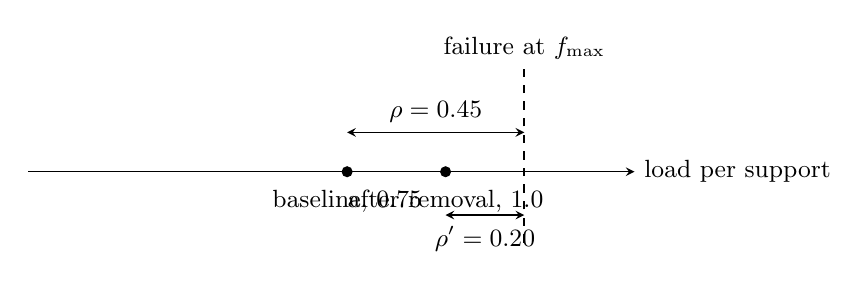
\begin{tikzpicture}[>=stealth, every node/.style={font=\small}]
\draw[->] (-0.3,0) -- (7.4,0) node[right] {load per support};
\draw[dashed,thick] (6,-0.9) -- (6,1.3) node[above] {failure at $f_{\max}$};
\fill (3.75,0) circle (2pt) node[below=3pt] {baseline, $0.75$};
\fill (5,0) circle (2pt) node[below=3pt] {after removal, $1.0$};
\draw[<->] (3.75,0.5) -- node[above] {$\rho=0.45$} (6,0.5);
\draw[<->] (5,-0.55) -- node[below=2pt] {} (6,-0.55);
\node at (5.5,-0.85) {$\rho'=0.20$};
\end{tikzpicture}
\caption{Both states lie on the safe side, so the coarse observable reads the same. The ablation moved the state toward the failure boundary and consumed reserve.}
\end{figure}

\subsection{A homeostat with a limited actuator}

The same phenomenon can be stated exactly in the homeostat, and doing so gives the margin a mechanism.

\begin{example}[Homeostat with actuator limit]\label{ex:limit}
Modify Example~\ref{ex:homeostat} by bounding the effort variable, $x_2\le x_2^{\max}$, with the controller acting as before until the bound is reached. Define the \emph{reserve} as $r=x_2^{\max}-x_2^0$, where $x_2^0=y^*-a$ is the baseline effort. Ablate a portion $\alpha a$ of the source, $x_1:a\mapsto a(1-\alpha)$.
\end{example}

\begin{proposition}[Reserve law]\label{prop:reserve}
In Example~\ref{ex:limit}, the required effort after ablation is $x_2^0+\alpha a$, and:
\begin{enumerate}[label=(\roman*)]
\item if $\alpha a\le r$, the chronic effect is $\Delta^\infty=0$ and the remaining margin (in effort units) is $r-\alpha a$;
\item if $\alpha a>r$, the actuator saturates at $x_2^{\max}$ and $\Delta^\infty=\alpha a-r$, with zero margin.
\end{enumerate}
The chronic effect is $\Delta^\infty(\alpha)=\max(0,\alpha a-r)$ and the compensation gap is $\kappa_\infty(\alpha)=\min(\alpha a,\,r)$. The margin lost equals the compensation gap.
\end{proposition}
\begin{proof}
The required effort to restore $Y=y^*$ with $x_1=a(1-\alpha)$ is $y^*-a(1-\alpha)=x_2^0+\alpha a$. The clipped relaxation is one-dimensional and converges monotonically to $\min(x_2^0+\alpha a,\,x_2^{\max})$. In case (i) the target is reachable, $Y=y^*$, and the margin is $x_2^{\max}-(x_2^0+\alpha a)=r-\alpha a$. In case (ii) $x_2=x_2^{\max}$ and $Y=a(1-\alpha)+x_2^{\max}=y^*-(\alpha a-r)$. The static effect is $\alpha a$, so $\kappa_\infty=\alpha a-\max(0,\alpha a-r)=\min(\alpha a,r)$, and in case (i) the margin lost is $r-(r-\alpha a)=\alpha a=\kappa_\infty$, with the same identity in case (ii) where the margin lost is $r$.
\end{proof}

Two conclusions follow. A null ablation of size $a$ establishes only $r\ge a$, a lower bound on the reserve, in the same way that Corollary~\ref{cor:rate} bounded the adaptation rate. And the null is the safe side of a cliff: a slightly larger ablation, or a slightly smaller reserve after some other loss, converts the silent null into a visible failure. A study that finds the ablation null has not found the system robust to that ablation in the sense of retaining its margin. It has found the system still on the safe side, with the margin reduced.

\begin{remark}[Combinatorial and metric margins]
Section~\ref{sec:profile} defined a combinatorial margin, the number of further components that can be removed. The metric margin $\rho$ here measures the distance to failure in state space. In the threshold system they coincide up to units, and in general the metric margin also registers erosion that removes no component, such as the loss of headroom in a saturating actuator.
\end{remark}

%------------------------------------------------------------------
\section{Non-Identifiability from Single Ablations}\label{sec:ident}
%------------------------------------------------------------------

The preceding sections gave examples. This section states the general result that makes the single-ablation null uninformative about architecture, and quantifies how uninformative.

Let a \emph{structure} on $K$ be a monotone Boolean function $\varphi:\{0,1\}^K\to\{0,1\}$ with $\varphi(\mathbf 1)=1$. It is determined by its family of minimal paths, an antichain $\mathcal A$ of subsets of $K$: $\varphi(z)=1$ iff $z$ contains some $A\in\mathcal A$. The \emph{single-ablation data} of $\varphi$ is the vector $(\varphi(\mathbf 1),\varphi(\mathbf 1-e_1),\dots,\varphi(\mathbf 1-e_n))$.

\begin{theorem}[Compatibility with many architectures]\label{thm:many}
Let $n\ge 4$ and $k=\lfloor n/2\rfloor$. The set of structures on $K$ whose single-ablation data is $(1,1,\dots,1)$ (a system that works and in which no single ablation matters) contains at least
\[
2^{N}-n\,2^{N/2},\qquad N=\binom{n}{k},
\]
pairwise distinct structures. These have distinct joint-ablation behavior.
\end{theorem}

The proof, given in Appendix~\ref{app:proofs}, constructs one structure for each subfamily of $k$-subsets that misses every component. A second theorem strengthens the point by bounding the number of ablations needed to \emph{determine} an unknown structure.

\begin{theorem}[Query lower bound]\label{thm:query}
Let $n\ge 3$ and $k=\lfloor n/2\rfloor$. Any deterministic procedure that determines an arbitrary structure on $K$ by querying values $\varphi(z)$ (equivalently, by performing ablations of $K\setminus z$) requires at least $\binom{n}{k}$ queries in the worst case, even when it is promised that every single-ablation is null.
\end{theorem}

Since $\binom{n}{\lfloor n/2\rfloor}\ge 2^n/(n+1)$, the number of queries grows exponentially in the number of components. The worst-case instances are those in which the informative ablations are the ones removing about half the system. The full proof is in Appendix~\ref{app:proofs}.

\begin{corollary}
Under a scalar binary observable, no polynomial-size collection of ablations determines the architecture of an arbitrary redundant system, and no collection of single ablations narrows the candidates beyond ``every component is non-necessary.''
\end{corollary}

\begin{remark}[Priors carry the inference]
Actual systems are not arbitrary. They are sparse, modular, approximately additive, spatially local, or otherwise structured. Under such priors, a modest number of ablations can be informative. The content of Theorems~\ref{thm:many} and~\ref{thm:query} is that the inference from ablation data to architecture is carried by these priors and not by the data alone, and that studies should say which priors they rely on. The same holds for the more general class of real-valued observables, which include the binary case.
\end{remark}

\begin{remark}[Generalization to $t$-wise ablations]
The $r$-out-of-$n$ threshold systems with $r\le n-t$ have all ablations of $t$ or fewer components null (Proposition~\ref{prop:below}). Hence a study restricted to $t$-wise ablations cannot distinguish any two structures whose minimal cuts all have size exceeding $t$. Theorem~\ref{thm:many} is the case $t=1$.
\end{remark}

%------------------------------------------------------------------
\section{The Converse: Non-Null Results Are Also Over-Read}\label{sec:converse}
%------------------------------------------------------------------

The logic of the essay applies in reverse. Just as $\Delta O\approx 0$ does not establish irrelevance, $\Delta O\gg 0$ does not establish that $C$ performs the lost function.

\paragraph{Destabilization.}
Removing a component can break a system for reasons unrelated to what the component contributed. The upper right cell of Table~\ref{tab:class} records this possibility: a null acute effect and a non-null reconfigured effect, caused by the adaptation itself misfiring. Removing a normalization layer from a trained network shifts activation statistics for all subsequent layers, producing catastrophic output whether or not the layer ``computed'' the function under study. The observed effect measures the system's dependence on the assumptions that the component upheld, which is not the same as its dependence on the component's function.

\paragraph{Diaschisis and distal effects.}
Lesion neuroscience has long recognized that damage to one region can depress activity in remote connected regions, a phenomenon for which von Monakow introduced the term diaschisis. A behavioral deficit after a lesion therefore does not localize the impaired function to the lesioned tissue. Lashley's classic experiments removing cortical tissue in rats and finding deficits that scaled with amount and not location were an early demonstration that lesion effects and function need not align~\cite{lashley1950}.

\paragraph{Deletion versus damage.}
Ablation replaces a component by its absence, which may differ from the component being present but broken, or replaced by a fixed default. A network unit set to zero is not the same intervention as the unit set to its mean activation or resampled from another input. The result depends on the replacement, and a study that reports only one has tested one counterfactual.

The symmetry is instructive. An ablation study reports the effect of an intervention and the system's response to it together. A null is the response cancelling the intervention, and a large effect is the response failing to cancel it. Neither isolates the intervention's contribution from the response.


%------------------------------------------------------------------
\section{Removal and Restoration: The Rebound Test}\label{sec:restore}
%------------------------------------------------------------------

Ablation is usually performed once and in one direction. The inverse experiment, restoring the component after the system has adapted to its absence, is informative in its own right, and it provides a certificate of compensation that requires neither joint ablations nor a chronic condition.

\begin{definition}[Ablate--restore cycle and rebound]
Ablate $C$ and let the system adapt for horizon $T$, then restore $\theta_C$ to its baseline value $\theta^0_C$ before the free coordinates have time to respond. The configuration immediately after restoration is $\bigl(\theta^0_C,\psi^a_T(\theta^0_{-C})\bigr)$. The \emph{rebound} is
\[
\rho_T(C)=d\Bigl(O(\theta^0),\ O\bigl(\theta^0_C,\psi^a_T(\theta^0_{-C})\bigr)\Bigr).
\]
\end{definition}

\begin{proposition}[Rebound certifies reconfiguration]\label{prop:rebound}
If $\rho_T(C)\ne0$ then $\psi^a_T(\theta^0_{-C})\ne\theta^0_{-C}$: the free coordinates moved during the ablation. Consequently the system is adaptive on the horizon $T$. In a non-adaptive system, $\rho_T=0$ for every $T$.
\end{proposition}
\begin{proof}
If $\psi^a_T(\theta^0_{-C})=\theta^0_{-C}$ the post-restoration configuration equals $\theta^0$ and $\rho_T=0$. The contrapositive is the first claim. For $V\equiv0$ the flow is the identity.
\end{proof}

The certificate is one-sided. A nonzero rebound proves adaptation. A zero rebound does not prove its absence, because the free coordinates may have moved in directions to which $O$ is blind at the baseline value of $\theta_C$.

\begin{proposition}[Rebound equals the compensation gap in the homeostat]\label{prop:reboundhomeo}
In Example~\ref{ex:homeostat}, the observable immediately after restoration is $Y=y^*+\kappa_T$, that is, an overshoot of exactly $\kappa_T=a(1-e^{-kT})$, and $\rho_T=\kappa_T$.
\end{proposition}
\begin{proof}
At the end of the ablation, $x_2=y^*-a\,e^{-kT}$ by Proposition~\ref{prop:horizon}. Restoring $x_1=a$ gives $Y=a+y^*-a\,e^{-kT}=y^*+a(1-e^{-kT})$.
\end{proof}

The rebound therefore reads the compensation gap directly: the amount by which the system over-corrects when the component returns equals the amount it had been compensating. In the regulated regime the ablation gives a null, and the restoration gives a spike whose height is the missing measurement.

\begin{remark}[Hysteresis]
If the adaptation dynamics have several attractors, as in a bistable switch, the ablate--restore cycle can end in a different basin from the one it started in, and the system after the cycle is not the system before it. Removal and restoration are then not inverse operations. This is a form of history dependence: the state after the cycle retains a consequence of a path no longer visible in the configuration.
\end{remark}

\begin{remark}[Asymmetry as curvature]
Even without adaptation, removal and addition differ for nonlinear responses. For a smooth scalar response $f$ at operating point $x$ and a step $\delta$, $\bigl[f(x+\delta)-f(x)\bigr]+\bigl[f(x-\delta)-f(x)\bigr]=f''(x)\,\delta^2+O(\delta^4)$. The sum of the effects of a step up and a step down of equal size estimates curvature, and it vanishes for a linear response. Ablation is a step down, and the missing step up is the missing half of a curvature measurement. A study restricted to ablation samples one side of the response.
\end{remark}

%------------------------------------------------------------------
%------------------------------------------------------------------
\section{Graded Interventions and Ablation Curvature}\label{sec:graded}
%------------------------------------------------------------------

An ablation replaces $\theta_C^0$ by $0_C$ in one step. Between these lies a family of partial ablations, and the observable along the family is a curve, not two numbers.

\begin{definition}[Graded ablation]
Fix a path $\alpha\mapsto c(\alpha)$ in $\Theta_C$ with $c(0)=\theta^0_C$ and $c(1)=0_C$; for a linear component $c(\alpha)=(1-\alpha)\theta^0_C$. The \emph{dose--response curve} at horizon $T$ is
\[
\alpha\longmapsto O_T(\alpha)=O\bigl(\Rop_T(S,\dox{\theta_C=c(\alpha)})\bigr),\qquad 0\le\alpha\le1 .
\]
\end{definition}

A single ablation samples the endpoints $O_T(0)$ and $O_T(1)$. The full curve exposes the slope $dO_T/d\alpha$ and the curvature $d^2O_T/d\alpha^2$, and it returns to the essay's opening distinction between a finite intervention and a derivative.

\subsection{Endpoint coincidence}

The sine example of Section~\ref{sec:setting} has a graded form: $O_T(\alpha)=\sin(2\pi\alpha)$ satisfies $O_T(0)=O_T(1)=0$ while the interior reaches $\pm1$. The next result says how much an interior excursion can be excluded by regularity.

\begin{proposition}[Interior bound from endpoints and smoothness]\label{prop:tent}
If $O_T(0)=O_T(1)$ and $O_T$ is $L$-Lipschitz in $\alpha$, then
\[
\sup_{0\le\alpha\le1}|O_T(\alpha)-O_T(0)|\ \le\ \frac L2 ,
\]
and the bound is attained by the tent function $O_T(\alpha)=L\min(\alpha,1-\alpha)$.
\end{proposition}
\begin{proof}
For each $\alpha$, $|O_T(\alpha)-O_T(0)|\le L\alpha$ and $|O_T(\alpha)-O_T(1)|\le L(1-\alpha)$. Since $O_T(0)=O_T(1)$ the left sides are equal, so the difference is at most $L\min(\alpha,1-\alpha)\le L/2$. The tent function meets it at $\alpha=1/2$.
\end{proof}

Without a Lipschitz bound, coinciding endpoints constrain nothing between them. With one, the interior is confined but not eliminated, and $L$ is a quantity the endpoint pair does not report.

\begin{figure}[ht]
\centering
\begin{minipage}{0.48\textwidth}
\centering
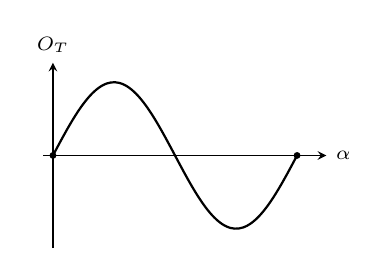
\begin{tikzpicture}[>=stealth, every node/.style={font=\scriptsize}, scale=0.62]
\draw[->] (-0.2,0) -- (5.6,0) node[right] {$\alpha$};
\draw[->] (0,-1.9) -- (0,1.9) node[above] {$O_T$};
\draw[thick,domain=0:1,samples=60,smooth] plot ({5*\x},{1.5*sin(360*\x)});
\fill (0,0) circle (2pt);
\fill (5,0) circle (2pt);
\end{tikzpicture}

\small(a) Equal endpoints, large interior.
\end{minipage}\hfill
\begin{minipage}{0.48\textwidth}
\centering
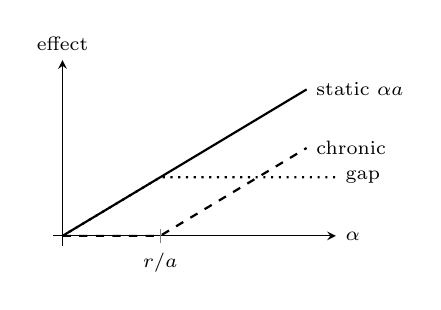
\begin{tikzpicture}[>=stealth, every node/.style={font=\scriptsize}, scale=0.62]
\draw[->] (-0.2,0) -- (5.6,0) node[right] {$\alpha$};
\draw[->] (0,-0.2) -- (0,3.6) node[above] {effect};
\draw[thick] (0,0) -- (5,3);
\node[right] at (5,3) {static $\alpha a$};
\draw[thick,dashed] (0,0) -- (2,0) -- (5,1.8);
\node[right] at (5,1.8) {chronic};
\draw[thick,dotted] (0,0) -- (2,1.2) -- (5.6,1.2);
\node[right] at (5.6,1.2) {gap};
\draw[gray] (2,-0.15) -- (2,0.15);
\node[below] at (2,-0.15) {$r/a$};
\end{tikzpicture}

\small(b) Static, chronic, and gap curves for the limited homeostat.
\end{minipage}
\caption{Dose--response curves. (a) Two endpoints can coincide while the path between them is highly non-null. (b) In the limited homeostat the chronic effect is flat until the reserve is exhausted and then rises with the static slope; the gap $\min(\alpha a,r)$ rises and then stays at the reserve.}
\end{figure}

\subsection{Dose--response in the limited homeostat}

Proposition~\ref{prop:reserve} gives the dose--response curves in closed form. The static curve is the line $\alpha a$. The chronic curve is $\max(0,\alpha a-r)$, flat until $\alpha=r/a$ and rising thereafter. The gap is $\min(\alpha a,r)$, rising and then constant at the reserve $r$.

\begin{proposition}[Local silence without global irrelevance]\label{prop:local}
In Example~\ref{ex:limit} with $a>r$, the chronic response has zero derivative at $\alpha=0$,
\[
\frac{d\Delta^\infty}{d\alpha}\Big|_{\alpha=0}=0,
\]
yet the ablation $\alpha=1$ is non-null, with effect $a-r>0$.
\end{proposition}
\begin{proof}
For $\alpha<r/a$ the chronic effect is identically zero, so its derivative at $0$ vanishes. At $\alpha=1$ it equals $a-r$.
\end{proof}

This is the exact converse of the opening proposition. Section~\ref{sec:setting} showed that $\Delta O\approx0$ does not imply $\partial O/\partial C=0$. Proposition~\ref{prop:local} shows that $\partial O/\partial C=0$ does not imply $\Delta O\approx0$. Neither the finite comparison nor the local derivative certifies irrelevance, and the dose--response curve is the object that contains both. The knee of the chronic curve identifies the reserve $r$, but only if the experiment reaches doses beyond it, which a physiological ablation may not. Where the reserve cannot be exhausted by removal, adding demand serves the same purpose.

\begin{remark}[Curvature and the missing half]
Section~\ref{sec:restore} observed that removal and addition together estimate curvature. The dose--response curve extended to $\alpha<0$ (an increase of the component) supplies the other side, and the second difference $O_T(\alpha)+O_T(-\alpha)-2O_T(0)$ estimates $O_T''(0)\alpha^2$ for small $\alpha$. In the limited homeostat the chronic curve has a corner at $\alpha=r/a$ and no curvature at $\alpha=0$, and the knee is visible only in the larger excursion.
\end{remark}

%------------------------------------------------------------------
\section{Statistical Certification of a Null}\label{sec:stat}
%------------------------------------------------------------------

The preceding sections concern what a null can mean when it is established. A prior question is when a null can be established at all. Failure to reject the hypothesis of no effect is not certification of no effect~\cite{altman1995}. What is needed is a test whose alternative hypothesis is the absence of a meaningful effect, and whose power is sufficient.

\subsection{Equivalence testing}

Let the ablation effect on trial $j$ be $y_j=\mu+\eta_j$ with $\eta_j$ independent, mean zero, and variance $\sigma^2$ known for simplicity. The claim to be certified is $|\mu|<\varepsilon$, where $\varepsilon$ is the smallest effect of scientific interest. The two one-sided tests procedure rejects the null hypothesis $|\mu|\ge\varepsilon$ at level $\alpha$ when both one-sided tests reject, which is equivalent to the $(1-2\alpha)$ confidence interval for $\mu$ lying inside $(-\varepsilon,\varepsilon)$~\cite{lakens2017}. In the known-variance case this is the condition
\[
|\bar y|<\varepsilon-z_{1-\alpha}\frac{\sigma}{\sqrt n},
\]
where $\bar y$ is the sample mean of $n$ trials and $z_{1-\alpha}$ the standard normal quantile.

\begin{proposition}[Minimum certifiable tolerance]\label{prop:mincert}
No number of favorable outcomes lets a study of $n$ trials certify equivalence to any tolerance $\varepsilon\le z_{1-\alpha}\sigma/\sqrt n$. In particular, if the true effect is exactly zero, the power to certify $|\mu|<\varepsilon$ is $2\Phi\bigl(\sqrt n\,\varepsilon/\sigma-z_{1-\alpha}\bigr)-1$, and power at least $1-\beta$ requires
\[
n\ \ge\ \Bigl(\frac{\sigma}{\varepsilon}\Bigr)^{2}\bigl(z_{1-\alpha}+z_{1-\beta/2}\bigr)^{2}.
\]
\end{proposition}
\begin{proof}
The certification condition requires $\varepsilon-z_{1-\alpha}\sigma/\sqrt n>|\bar y|\ge0$, impossible unless $\varepsilon>z_{1-\alpha}\sigma/\sqrt n$. When $\mu=0$, $\bar y\sim N(0,\sigma^2/n)$, so the probability that $|\bar y|<c$ with $c=\varepsilon-z_{1-\alpha}\sigma/\sqrt n$ is $2\Phi(c\sqrt n/\sigma)-1$, which is the stated power. Requiring this to be at least $1-\beta$ gives $c\sqrt n/\sigma\ge z_{1-\beta/2}$, and rearranging yields the bound on $n$.
\end{proof}

For $\alpha=0.05$ and $\beta=0.2$ the factor $(z_{0.95}+z_{0.90})^2$ is about $8.56$, so $n\gtrsim 8.56\,(\sigma/\varepsilon)^2$.

\begin{center}
\small
\begin{tabular}{cc}
\toprule
$\varepsilon/\sigma$ & Trials $n$ needed\\
\midrule
$1$ & $9$\\
$1/2$ & $35$\\
$1/4$ & $138$\\
$1/10$ & $857$\\
\bottomrule
\end{tabular}
\end{center}

The cost grows as the square of the required precision. A tolerance of a tenth of the trial-to-trial standard deviation requires hundreds of trials for a single component. Ablation studies of large systems commonly average over a handful of seeds or inputs, so their nulls certify only tolerances comparable to the noise itself.

\subsection{Many components}

Screening $m$ components for nulls is a family of $m$ equivalence claims. Each is an intersection-union test, so no correction is required within a component, but the claims must be corrected across components if a statement about all of them is made. With Bonferroni adjustment $\alpha\to\alpha/m$, the constant $(z_{1-\alpha}+z_{1-\beta/2})^2$ rises from $8.56$ to about $20.9$ for $m=100$ (using $z_{1-\alpha/m}\approx3.29$), a factor of roughly $2.4$. Testing all pairs of $n$ components multiplies $m$ by $\binom n2$ and the required sample by a further logarithmic factor, which is one more reason the interaction structure is rarely screened.

\begin{remark}[Tolerance is a scientific choice]
The tolerance $\varepsilon$ must be fixed from the scientific question, as the smallest effect of interest, before data are collected. Choosing $\varepsilon$ after the fact to match the achievable precision reproduces the original error in different notation: the claim then reports the resolution of the experiment and not the behavior of the system.
\end{remark}

%------------------------------------------------------------------
\section{Consequences for Interpretation and Reporting}\label{sec:practice}
%------------------------------------------------------------------

\subsection{Domains}

\paragraph{Neural network interpretability.}
Circuit-level analyses of transformers have identified backup components that take over when primary ones are ablated. In the analysis of indirect object identification in a small language model, ablating the main name-moving heads was found to activate other heads with a similar role~\cite{wang2022}. The phenomenon of downstream layers adjusting to compensate for an ablated layer has been described as self-repair and studied as a general effect in language models~\cite{mcgrath2023}. Earlier work on single-unit ablation asked how much individual units matter for generalization and found that units with strong selectivity were not more important than others~\cite{morcos2018}, which is a form of the null-versus-importance gap in a different vocabulary. In all these cases, a component can fail an ablation test while being causally central, and any inference from ablation to mechanism should be paired with a test of the compensation hypothesis.

\paragraph{Genetics.}
The discrepancy between genetic mutants and acute knockdowns has been attributed in several cases to transcriptional adaptation, where mutant transcripts trigger upregulation of related genes~\cite{rossi2015,elbrolosy2019}. The knockout phenotype is then the phenotype of $\Rop_\infty$ and the knockdown is closer to $\Rop_0$. Reporting both is the experimental analogue of the pair $(\Delta^0,\Delta^\infty)$ in Table~\ref{tab:class}.

\paragraph{Structures and load paths.}
Structural engineering already contains the concept that nothing happening to the coarse observable, the structure standing, is compatible with substantial reconfiguration of the internal load paths. The reserve capacity of redundant members is a designed compensation, and its consumption is invisible to an inspector who looks only at whether the building stands.

\paragraph{Institutions.}
Removing a role, rule, or office from an organization and finding that outcomes are unchanged is routinely read as evidence that the item was superfluous. The same logic applies: duties may have been reassigned, informal channels may have absorbed the function, and the reconfiguration may have a cost paid elsewhere in the system.

\subsection{A minimal reporting standard}

The following items are proposed as a minimum for any study whose conclusion depends on a null ablation. They are listed in Appendix~\ref{app:checklist} in checklist form.

\begin{enumerate}[label=\textbf{R\arabic*.}]
\item \textbf{Intervention type and replacement value.} State how the component was removed (zeroed, mean-ablated, resampled, deleted, degraded) and whether other choices were tested.
\item \textbf{Adaptation horizon.} State whether the system had time to reconfigure, and report at least one acute and one chronic condition when both are feasible.
\item \textbf{Observable and resolution.} State the observable, its resolution, and the tolerance $\varepsilon$ used to call an effect null, with a justification. Use an equivalence test rather than failure to reject when claiming absence of an effect.
\item \textbf{Operating conditions.} State the regime tested and whether saturation, ceiling, or floor effects are plausible in it. Vary the background where possible.
\item \textbf{Joint ablations.} Report ablations of pairs among the plausible compensators, at least those suggested by the architecture. State the largest joint size tested.
\item \textbf{Effort variables.} Report the state of the non-regulated variables after ablation. A null on the regulated variable accompanied by shifts in effort variables is a compensation, not an absence of function.
\item \textbf{Claim language.} Replace ``$C$ is not necessary'' or ``$C$ does nothing'' by the exact claim: ``no effect exceeding $\varepsilon$ on $O$ under conditions $X$ at horizon $T$ for interventions of type $I$.''
\end{enumerate}

None of these is burdensome for a single study, and they convert the null from a claim of absence into a bounded statement that other work can build on or contradict.

%------------------------------------------------------------------
\section{Designing for Informative Nulls}\label{sec:design}
%------------------------------------------------------------------

The reporting standard of Section~\ref{sec:practice} governs how existing experiments are described. The results above also bear on how systems and experiments should be built so that a future null carries information. Five principles follow from the theory.

\begin{enumerate}[label=\textbf{D\arabic*.}]
\item \textbf{Expose the effort variables.} Proposition~\ref{prop:effort} places the information about a compensated ablation in the free coordinates, and Theorem~\ref{thm:tomo} shows that observing them turns single ablations into a reconstruction. A system that logs only its regulated output discards this information at the source. Recording the state of backup pathways is cheap when planned and often impossible retrospectively.
\item \textbf{Provide ablation as a first-class interface.} An intervention layer that supports several replacement modes (zero, mean, resampled, and restored) and several horizons converts the question ``what did $C$ do'' into a family of measurements. This includes the ability to restore, since the rebound test of Section~\ref{sec:restore} depends on it.
\item \textbf{Instrument the reserve.} The tolerance margin of Proposition~\ref{prop:margin} is a property of the system that no single ablation reveals, but it can be monitored. In structural health monitoring, gauges on redundant members detect that one has failed even though the structure stands, because the survivors' loads shift by a predictable factor $n/(n-1)$. The analogous telemetry for other systems is the load on backup components, and a sudden change in it is a signal that reserve has been consumed.
\item \textbf{Test on fresh specimens or restore between tests.} Proposition~\ref{prop:consume} shows that successive ablations on one specimen test progressively weaker systems. Independent replicates, or ablate--restore cycles that return the system to baseline before the next test, keep each ablation a test of the intact system.
\item \textbf{Select ablations adaptively.} With a budget of ablations, choose the next intervention using the residuals of the previous ones. Theorem~\ref{thm:query} says the worst case is exponential, but under sparsity priors adaptive selection can approach the linear cost seen in Theorem~\ref{thm:tomo}, where $n$ single ablations suffice.
\end{enumerate}

None of these principles requires knowledge of the architecture in advance. They amount to arranging for the system to keep, and for the experimenter to see, the variables into which a silent ablation transfers its information.

%------------------------------------------------------------------
\section{Connections to Broader Frameworks}\label{sec:framework}
%------------------------------------------------------------------

The formal results above are self-contained. Several frameworks developed elsewhere in this research program address the same structure in a different vocabulary, and the correspondences are recorded briefly.

\paragraph{Refusal in SpherePOP.}
In the SpherePOP formalism the REFUSE primitive is not mere nonparticipation. Refusing one route can change which route becomes admissible, so the effect of a refusal is not the effect of the route being absent from an otherwise unchanged set of routes. This is the operator picture of Theorem~\ref{thm:notsub}: refusing $C$ is an intervention followed by a change in the admissibility structure of what remains, and the two must be distinguished.

\paragraph{Residuals as topology probes.}
In the residual-and-admissibility line of work, the remainder after a computation is treated as information and not as error. The residual after ablation plays this role. It is the trace left in the surviving components, and it is a probe of the topology of what remains. The effort variables of Proposition~\ref{prop:effort} and the survivor strains of the load-path example are instances.

\paragraph{Charts in HOLOcoord.}
An element cannot be assigned significance from its isolated coordinate, because removing it changes the transition relations among the surviving charts. This is the statement that the local role of a component is defined relative to the atlas in which it sits, and that deleting it produces a different atlas. The distinction between $S-C$ and $\Rop(S,\dox{C=0})$ is a distinction between the atlas with a chart deleted and the atlas re-glued.

\paragraph{History in MEM|8.}
Persistence of a rendered state after deletion does not establish the absence of historical dependence. The state can retain consequences of a path that is no longer locally visible. In the language of this essay, the observable is unchanged because the effect has moved into an unobserved variable, and the history that produced that variable is what the null conceals.

These correspondences are offered as orientation. The essay does not depend on them, and each reduces, for present purposes, to the theorems above.

%------------------------------------------------------------------
\section{Objections and Replies}\label{sec:objections}
%------------------------------------------------------------------

\paragraph{Objection 1: Experimentalists already know this.}
The caution is widely voiced, and terms such as compensation, redundancy, and backup pathway are standard. The claim of this essay is narrower. The caution is rarely operationalized: reports seldom state the horizon, the tolerance, the replacement value, or whether joint ablations were run, and conclusions are still phrased as absence. Sections~\ref{sec:time} through~\ref{sec:stat} give the quantities that would turn the caution into a reportable result: a rate bound (Corollary~\ref{cor:rate}), a margin (Proposition~\ref{prop:margin}), a rebound (Proposition~\ref{prop:reboundhomeo}), and a certifiable tolerance (Proposition~\ref{prop:mincert}).

\paragraph{Objection 2: Compensation is a rare special case.}
How common compensation is in a given class of systems is an empirical question, and the essay takes no position on the frequency. The point is logical. The inference from null to irrelevance is licensed only if compensation, saturation, degeneracy, coarseness, and level-set coincidence have been excluded, and their frequency in a class of systems is what determines how often the inference fails. Degeneracy and redundancy are widely regarded as pervasive in biological and engineered systems~\cite{edelman2001}. The experiments proposed here, a second horizon, a joint ablation, a rebound, estimate the frequency for the system at hand rather than assuming it.

\paragraph{Objection 3: A non-null effect still proves necessity.}
It proves necessity at the tested horizon, for the tested replacement, under the tested conditions, and only if destabilization and distal effects are excluded (Section~\ref{sec:converse}). The symmetry of the argument is the reason the essay treats both directions. The claim is not that ablation is uninformative but that it reports the combined effect of an intervention and a response, and that the two must be separated by design.

\paragraph{Objection 4: This proves too much. If nulls cannot be trusted, nothing can.}
The argument does not say nulls cannot be trusted. It says which claims a null can support, and it gives those claims a precise form: no effect exceeding $\varepsilon$ on $O$ under conditions $X$ at horizon $T$, certified by an equivalence test with stated power. Such claims are useful, they can be combined across studies, and they can be strengthened by the additional experiments the essay describes. In the linear case, Theorem~\ref{thm:tomo} shows that nulls can be turned from an uncertainty into a complete measurement when the observable is rich enough.

\paragraph{Objection 5: The exponential lower bound is a worst-case result.}
It is. Theorems~\ref{thm:many} and~\ref{thm:query} construct adversarial families, and real systems are structured. The remark following them states that priors such as sparsity, modularity, and locality carry the inference in practice. The result is offered as a demand that these priors be stated, since without them the data underdetermine the architecture, and as a warning that the underdetermination is severe when the observable is a single bit.

\paragraph{Objection 6: Adaptation is a nuisance, and the frozen counterfactual $S-C$ is what is wanted.}
That depends on the question. If the question is mechanistic, what $C$ contributes at the operating point, then $\Delta^0$ is the relevant quantity and the acute regime is appropriate. If the question concerns robustness, what happens to the system when $C$ is lost, then $\Delta^\infty$ is relevant. The same intervention answers both questions when the horizon is varied, and the gap between the two answers is the compensation of Lemma~\ref{lem:gap}. Treating one question's answer as the other's is the error under discussion.

%------------------------------------------------------------------
%------------------------------------------------------------------
\section{Invariance Is Relative to an Observer}\label{sec:observer}
%------------------------------------------------------------------

The preceding sections have repeatedly changed the observable in order to change the verdict: a scalar output versus the effort variables, a coarse pass/fail measure versus a fine one, an endpoint versus a curve. These are instances of one relation among observers.

\subsection{Refinement}

\begin{definition}[Observers and refinement]
An observer is a map $O:\Theta\to Y$. The observer $O_2$ \emph{refines} $O_1$ if $O_1=f\circ O_2$ for some map $f$. Then $O_1$ is coarser.
\end{definition}

\begin{proposition}[Factorization criterion]\label{prop:factor}
$O_1$ factors through $O_2$ if and only if $\sim_{O_2}\ \subseteq\ \sim_{O_1}$, that is, $[\theta]_{O_2}\subseteq[\theta]_{O_1}$ for every $\theta$.
\end{proposition}
\begin{proof}
If $O_1=f\circ O_2$ and $O_2(\theta)=O_2(\theta')$ then $O_1(\theta)=O_1(\theta')$. Conversely, if the inclusion holds, define $f(O_2(\theta))=O_1(\theta)$. This is well defined because $O_2(\theta)=O_2(\theta')$ implies $O_1(\theta)=O_1(\theta')$, and it defines $f$ on the image of $O_2$.
\end{proof}

\begin{corollary}[Silence is monotone under coarsening]\label{cor:mono}
If $O_2$ refines $O_1$ and an ablation is exactly null for $O_2$, it is exactly null for $O_1$. The converse fails: an ablation can be null for $O_1$ and not for $O_2$. If $f$ is $1$-Lipschitz, the same holds for $\varepsilon$-nulls.
\end{corollary}
\begin{proof}
$\Rop_T\sim_{O_2}\theta^0$ implies $\Rop_T\sim_{O_1}\theta^0$ by the proposition. For the $\varepsilon$ version, $d_1(O_1(\Rop_T),O_1(\theta^0))=d_1(f(O_2(\Rop_T)),f(O_2(\theta^0)))\le d_2(O_2(\Rop_T),O_2(\theta^0))$. For the failure of the converse, take the homeostat with $O_1=Y$ and $O_2=(Y,x_2)$: after chronic ablation $\Delta O_1=0$ and $\Delta O_2=a\ne0$.
\end{proof}

\begin{figure}[ht]
\centering
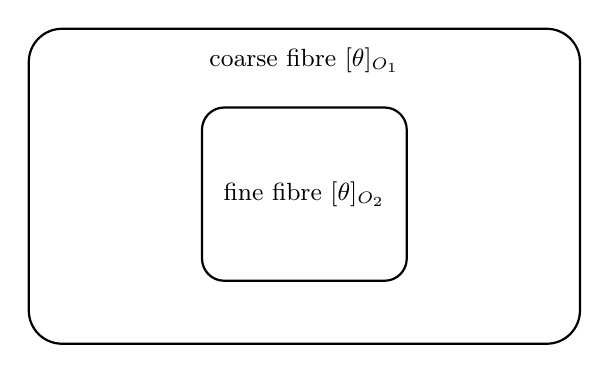
\begin{tikzpicture}[>=stealth, every node/.style={font=\small}]
\draw[rounded corners=12pt,thick] (0,0) rectangle (7,4);
\draw[rounded corners=8pt,thick] (2.2,0.8) rectangle (4.8,3.0);
\node at (3.5,3.6) {coarse fibre $[\theta]_{O_1}$};
\node at (3.5,1.9) {fine fibre $[\theta]_{O_2}$};
\end{tikzpicture}
\caption{Refining the observer shrinks the equivalence class. Any ablation that stays within the fine fibre is invisible to both observers; one that leaves it but stays in the coarse fibre is visible only to $O_2$.}
\end{figure}

Every observer is a partition of $\Theta$, and refinement is the partition order. An ablation is null for an observer when the intervention stays within one block, and coarser observers have larger blocks. This is the abstract statement that lies under the earlier results about resolution: a scalar is a very coarse observer of a network, and the survivor vector is a fine one.

\subsection{Richer observation shrinks the compatible set}

The same order acts on the inference from data to architecture. Let $\mathcal S$ be a class of candidate architectures and let $F_1:\mathcal S\to\mathcal D_1$ be an experimental protocol, mapping an architecture to the data it would produce.

\begin{proposition}[Refined protocols shrink compatible sets]\label{prop:shrink}
If $F_2=(F_1,G)$ appends further measurements $G$ to a protocol $F_1$, then for every observed datum $d_2=(d_1,g)$,
\[
\{S\in\mathcal S:\ F_2(S)=d_2\}\ \subseteq\ \{S\in\mathcal S:\ F_1(S)=d_1\}.
\]
\end{proposition}
\begin{proof}
Any $S$ with $F_2(S)=(d_1,g)$ has $F_1(S)=d_1$.
\end{proof}

The proposition is elementary and it is the abstract form of the contrast between Theorems~\ref{thm:many} and~\ref{thm:tomo}. Under the scalar protocol the compatible set contains at least $2^N-n2^{N/2}$ structures. After the protocol is refined to the survivor vectors, the compatible set in the symmetric linear class is a single architecture. Everything between is a monotone shrinking of the set as observers are added.

\subsection{No privileged observer}

Two ablation studies of the same system with different observers can both be correct and disagree, exactly as two studies at different horizons can (Corollary~\ref{cor:disagree}). The disagreement is a comparison of partitions. A report should state its observer, and the reporting standard of Section~\ref{sec:practice} already does so under R3. The additional recommendation from this section is to report, where possible, a finer observer alongside the coarse one, because Corollary~\ref{cor:mono} guarantees that the finer observer can only reduce silence.

%------------------------------------------------------------------
\section{From Null Results to Structural Tomography}\label{sec:tomography}
%------------------------------------------------------------------

Section~\ref{sec:ident} showed that scalar single-ablation data cannot identify architecture. Section~\ref{sec:necessity} showed that the information discarded by a null lives in the residual, that is, in the state of the surviving components. This suggests that the negative result is an artifact of the coarse observable, and that with a richer observable a sequence of ablations and their compensations can reconstruct the hidden network. This section proves a case in which that is exactly true.

\subsection{A linear model}

Consider a linear equilibrium network. Let $K$ be a real symmetric positive definite $n\times n$ matrix (a conductance, stiffness, or coupling matrix), let $u\in\R^n$ be a known input, and let $x=Gu$ with $G=K^{-1}$ be the equilibrium state. Ablating node $i$ clamps $x_i=0$ and removes the node's equation, which leaves the reduced system
\[
K_{-i,-i}\,x^{(i)}=u_{-i},
\]
where $K_{-i,-i}$ is the principal submatrix omitting row and column $i$. Let $x_{-i}$ denote the baseline state restricted to the other nodes. The following identity describes the residual.

\begin{lemma}[Ablation residual]\label{lem:residual}
The residual $r^{(i)}=x^{(i)}-x_{-i}$ satisfies
\[
r^{(i)}=K_{-i,-i}^{-1}K_{-i,i}\,x_i=-\frac{G_{-i,i}}{G_{ii}}\,x_i .
\]
\end{lemma}
\begin{proof}
The baseline equations restricted to rows $-i$ read $K_{-i,-i}x_{-i}+K_{-i,i}x_i=u_{-i}$. Subtracting $K_{-i,-i}x^{(i)}=u_{-i}$ gives $K_{-i,-i}(x^{(i)}-x_{-i})=K_{-i,i}x_i$, which is the first equality. For the second, the identity $KG=I$ restricted to the block of rows $-i$ and column $i$ gives $K_{-i,-i}G_{-i,i}+K_{-i,i}G_{ii}=0$, so $K_{-i,-i}^{-1}K_{-i,i}=-G_{-i,i}/G_{ii}$.
\end{proof}

The residual is a multiple of a column of the Green's function $G$. It is the response of the surviving network to the removal of node $i$'s coupling, and it points along the direction in which node $i$ was connected to the rest.

\subsection{Identifiability}

\begin{theorem}[Linear structural tomography]\label{thm:tomo}
Let $K$ be symmetric positive definite with $G=K^{-1}$ having no zero entries, let $u$ be known, and suppose the baseline state $x=Gu$ has $x_i\ne 0$ for all $i$. If one observes $x$ and the ablated states $x^{(i)}$ for all $i=1,\dots,n$, then $K$ is uniquely determined.
\end{theorem}
\begin{proof}
By Lemma~\ref{lem:residual}, $r^{(i)}=-(G_{-i,i}/G_{ii})x_i$, so since $x_i\ne 0$ the normalized column $\tilde g_i:=G_{-i,i}/G_{ii}=-r^{(i)}/x_i$ is determined by observations. Thus $G_{ji}=G_{ii}\tilde g_i[j]$ for all $j\ne i$. Symmetry of $G$ gives $G_{ii}\tilde g_i[j]=G_{jj}\tilde g_j[i]$, and since $G$ has no zero entries both $\tilde g_i[j]$ and $\tilde g_j[i]$ are nonzero, so
\[
\frac{G_{jj}}{G_{ii}}=\frac{\tilde g_i[j]}{\tilde g_j[i]}.
\]
Taking $i=1$ determines $d_j:=G_{jj}/G_{11}$ for all $j$ (with $d_1=1$). Then $G=G_{11}\tilde D$ where $\tilde D_{ji}=d_i\tilde g_i[j]$ for $j\ne i$ and $\tilde D_{ii}=d_i$ are known. Finally $x=Gu=G_{11}\tilde Du$; since $x_1\ne0$, $(\tilde Du)_1\ne 0$ and $G_{11}=x_1/(\tilde Du)_1$. Thus $G$ is determined, and $K=G^{-1}$.
\end{proof}


\begin{figure}[ht]
\centering
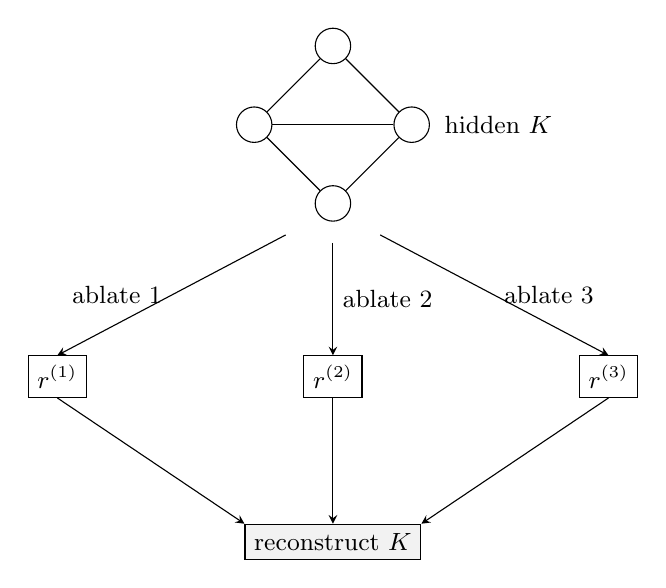
\begin{tikzpicture}[>=stealth, every node/.style={font=\small}]
\node[draw,circle,minimum size=0.45cm] (n1) at (0,1) {};
\node[draw,circle,minimum size=0.45cm] (n2) at (-1,0) {};
\node[draw,circle,minimum size=0.45cm] (n3) at (1,0) {};
\node[draw,circle,minimum size=0.45cm] (n4) at (0,-1) {};
\draw (n1) -- (n2) -- (n4) -- (n3) -- (n1);
\draw (n2) -- (n3);
\node at (2.1,0) {hidden $K$};
\node[draw,rectangle] (r1) at (-3.5,-3.2) {$r^{(1)}$};
\node[draw,rectangle] (r2) at (0,-3.2) {$r^{(2)}$};
\node[draw,rectangle] (r3) at (3.5,-3.2) {$r^{(3)}$};
\draw[->] (-0.6,-1.4) -- node[left,pos=0.5] {ablate $1$} (r1.north);
\draw[->] (0,-1.5) -- node[right,pos=0.5] {ablate $2$} (r2.north);
\draw[->] (0.6,-1.4) -- node[right,pos=0.5] {ablate $3$} (r3.north);
\node[draw,rectangle,fill=gray!10] (rec) at (0,-5.3) {reconstruct $K$};
\draw[->] (r1.south) -- (rec.north west);
\draw[->] (r2.south) -- (rec.north);
\draw[->] (r3.south) -- (rec.north east);
\end{tikzpicture}
\caption{Structural tomography. Each single ablation of the hidden network produces a residual vector $r^{(i)}$ proportional to a column of the Green's function. Under the hypotheses of Theorem~\ref{thm:tomo}, the collection of residuals determines $K$.}
\end{figure}

Theorem~\ref{thm:tomo} contrasts with Theorems~\ref{thm:many} and~\ref{thm:query}. In the latter, the observable is a single bit and $n$ single ablations reveal nothing about structure. In the former, the observable is the full survivor vector, and $n$ single ablations reveal everything. The two theorems bracket the role of resolution: the null on the scalar is uninformative because the information has moved into variables the scalar does not record. Whenever the survivors are recorded, the nulls become a measurement.

\begin{example}[Parallel supports revisited]
Return to $n$ identical parallel supports under load $W$. Removing one leaves $W/(n-1)$ per survivor against baseline $W/n$, a ratio $n/(n-1)$. With ratios $2,\ 3/2,\ 4/3,\ 6/5$ for $n=2,3,4,6$ respectively, a single measured strain ratio identifies the number of supports, although the coarse observable (the deck stands) is silent. The single ablation is a null in the binary observable and a full measurement of $n$ in the strain observable.
\end{example}

\subsection{Sequences of interventions}

The result concerns single ablations in a linear symmetric model. The wider proposal it motivates is that sequences of interventions and the compensations they induce can serve as a form of tomography for invisible networks: a family of ablations $\{a_1,a_2,\dots\}$ paired with the residuals $\{r_1,r_2,\dots\}$ constrains the interaction structure, in the way that a family of projections constrains an image. Several questions arise.

\begin{itemize}[leftmargin=1.4em]
\item \textbf{Nonlinearity.} Lemma~\ref{lem:residual} has a first-order analogue near an operating point of a nonlinear system, with $G$ replaced by the inverse Jacobian. How large a perturbation is admissible before the local linearization fails, and can residual asymmetry between an ablation and its inverse estimate the nonlinearity?
\item \textbf{Adaptation.} When the system adapts, the residual depends on the horizon $T$. The time course of the residual, rather than its endpoint, may encode the adaptation dynamics $V$, so that the family $\Rop_T$ is itself an observable of the hidden architecture.
\item \textbf{Adaptive design.} Given a budget of ablations, which sequence maximizes information? By Theorem~\ref{thm:query} the worst-case cost is exponential, but under sparsity priors adaptive selection of the next ablation from the previous residuals may achieve far better.
\item \textbf{Noise.} Identifiability under measurement noise depends on the conditioning of $K$ and of its principal submatrices, and the noise tolerance of the reconstruction is an open quantity.
\end{itemize}

These questions belong to a sequel whose organizing image is the load path that no one drew: an internal route for force, signal, or influence, invisible in the finished structure and recoverable only from the pattern of how the structure responds when pieces are taken away.

%------------------------------------------------------------------
%------------------------------------------------------------------
\section{Preserved Distinctions}\label{sec:principle}
%------------------------------------------------------------------

The results of the essay can be summarized as a principle about when distinctions may be discarded.

\begin{quote}
\textbf{Preserve distinctions before composing them.}
\end{quote}

A distinction between two states may be erased by an observer (a coarse output, an average, a threshold) or by a composition of operations (aggregating before comparing, quantizing before storing). Once erased at one level it is recoverable only if some other observer still separates the states. The following instances have appeared above.

\paragraph{Refusal is not absence.}
Removing a component by subtraction ($\Rop_0$) and refusing it as an intervention ($\Rop_T$) are different operations, because the latter is followed by reconfiguration of what remains (Theorem~\ref{thm:notsub}). The two must not be composed into a single notion of ``the system without $C$''.

\paragraph{Persistence is not truth.}
That the observable persists after deletion is a fact about the observer, not about the state. The unchanged reading is compatible with a changed configuration, a running cost, and a reduced margin (Section~\ref{sec:quotient}). Persistence of a value certifies nothing about the underlying history.

\paragraph{Recovery is not invention.}
Under the survivor-vector observer in the symmetric linear class, the compatible architecture is unique and the reconstruction is a function of the data alone (Theorem~\ref{thm:tomo}): this is recovery. Under the scalar observer the compatible set is exponentially large (Theorem~\ref{thm:many}), and any single architecture selected from it is selected by a prior: this is invention. The same procedure can be either, depending on the observer.

More abstractly, observational equivalence is not identity:
\[
O(x)=O(y)\ \not\Longrightarrow\ x=y .
\]

\begin{proposition}[Recoverability of distinctions]\label{prop:recover}
Let $O_1,\dots,O_J$ be the available observers. A distinction $\theta\ne\theta'$ is recoverable if and only if some $O_j$ has $O_j(\theta)\ne O_j(\theta')$. All distinctions are recoverable if and only if $\bigcap_j\sim_{O_j}$ is the identity relation, that is, the joint observer $(O_1,\dots,O_J)$ is injective. Composing an observer with any map $q$ can only enlarge the erased relation: $\sim_O\subseteq\sim_{q\circ O}$, with strict inclusion whenever $q$ identifies two values in the image of $O$.
\end{proposition}
\begin{proof}
The first two claims restate the definitions. If $O(\theta)=O(\theta')$ then $q(O(\theta))=q(O(\theta'))$, giving the inclusion. If $q$ identifies two distinct values $O(\theta_1)\ne O(\theta_2)$ then $\theta_1\sim_{q\circ O}\theta_2$ but $\theta_1\not\sim_O\theta_2$.
\end{proof}

A system is interpretable only insofar as the distinctions erased at one level remain recoverable at another. The practical rule that follows from the proposition is a rule about order: record the un-aggregated state (effort variables, residuals, the state of backups) and the intervention before averaging over seeds, inputs, or specimens, and before thresholding to a pass/fail outcome. Composition can be done afterward from the record. It cannot be undone.

%------------------------------------------------------------------
\section{Conclusion}
%------------------------------------------------------------------

The sentence ``we removed $C$, and nothing happened'' reports that a finite intervention left a measured observable within tolerance. That is all it reports. It does not report that the sensitivity vanishes, because a finite step is not a derivative and the step may land on the same level set. It does not report that $C$ was redundant, because the system may have re-supplied $C$'s contribution rather than possessed a duplicate. It does not report that the system minus $C$ was measured, because in adaptive systems the measured object is $\Rop(S,\dox{C=0})$, the output of a reconstruction, and $S-C$ is only the frozen counterfactual of it.

The positive content of the null is the compensatory transformation of Corollary~\ref{cor:hidden}, together with the compensation gap of Lemma~\ref{lem:gap}, which bounds from below how much the system did in response. The information lost by a scalar readout is not destroyed. It is relocated into effort variables, into joint ablations, into the time course of the residual, and into the state of the survivors, where Theorem~\ref{thm:tomo} shows it can, in a tractable case, be fully recovered.

The geometric reading unifies the results. A null ablation is a return of the trajectory to the observational fibre of the baseline, and an experiment that records only the observable sees the quotient by that fibration. In these terms, \emph{invariance is not absence of change; it is change constrained to remain invisible under a specified observation map.} Output invariance does not imply configuration invariance, cost invariance (Proposition~\ref{prop:cost}), or margin invariance (Proposition~\ref{prop:reserve}), and a zero local derivative does not imply a null finite ablation (Proposition~\ref{prop:local}), just as a null finite ablation does not imply a zero derivative.

The added structure of timing, margin, and rebound supplies further handles on the same phenomenon. A null at a single horizon bounds the adaptation rate from below (Corollary~\ref{cor:rate}), and the disagreement between studies at different horizons is a measurement of the crossover time. The whole ablation profile reveals the tolerance margin that single ablations conceal, and random ablation can miss a small cut with overwhelming probability (Proposition~\ref{prop:random}). The rebound after restoration reads the compensation gap directly (Proposition~\ref{prop:reboundhomeo}). And a null can be certified only at tolerances the noise level and sample size permit (Proposition~\ref{prop:mincert}).

Two consequences follow for practice. Claims of absence should be written as bounded statements of the form given in the reporting standard, with tolerance, horizon, replacement, and conditions stated. And the null result should be treated as the beginning of an experiment: the natural next measurements are the joint ablation, the second horizon, and the residual, each of which converts a silence into a finding.

The general principle, stated in Section~\ref{sec:principle}, is to preserve distinctions before composing them. Observational equivalence is not identity, refusal is not absence, persistence is not truth, and recovery is not invention. A system remains interpretable only insofar as the distinctions erased at one level remain recoverable at another.

%------------------------------------------------------------------
\appendix
\section{Proofs of Theorems~\ref{thm:many} and~\ref{thm:query}}\label{app:proofs}
%------------------------------------------------------------------

\begin{proof}[Proof of Theorem~\ref{thm:many}]
Let $n\ge 4$, $k=\lfloor n/2\rfloor$, and let $\binom{[n]}{k}$ denote the $k$-subsets of $K=[n]$, so $|\binom{[n]}{k}|=N$. For a subfamily $\mathcal F\subseteq\binom{[n]}{k}$ define $\varphi_{\mathcal F}(z)=1$ iff $z\supseteq A$ for some $A\in\mathcal F$. All members of $\mathcal F$ have the same size, hence form an antichain, and $\varphi_{\mathcal F}$ is monotone. Distinct subfamilies yield distinct functions: for $A\in\binom{[n]}{k}$ we have $\varphi_{\mathcal F}(\mathbf 1_A)=1$ iff $A\in\mathcal F$, since a $k$-set contains a member of $\mathcal F$ only if it equals that member.

Call $\mathcal F$ \emph{good} if for every $i\in[n]$ some $A\in\mathcal F$ has $i\notin A$. If $\mathcal F$ is good then $\mathcal F\ne\emptyset$, so $\varphi_{\mathcal F}(\mathbf 1)=1$, and for each $i$ the set $[n]\setminus\{i\}$ contains some $A\in\mathcal F$, so $\varphi_{\mathcal F}(\mathbf 1-e_i)=1$. Thus every good subfamily has single-ablation data $(1,\dots,1)$.

It remains to count good subfamilies. A subfamily is \emph{not} good iff there is $i$ with $i\in A$ for every $A\in\mathcal F$, that is, $\mathcal F\subseteq\{A\in\binom{[n]}{k}:i\in A\}$. This set has $\binom{n-1}{k-1}$ elements, so at most $2^{\binom{n-1}{k-1}}$ subfamilies are contained in it. By a union bound over $i$, the number of subfamilies that are not good is at most $n\,2^{\binom{n-1}{k-1}}$. Now $\binom{n-1}{k-1}=\frac{k}{n}\binom nk\le N/2$ because $k=\lfloor n/2\rfloor\le n/2$. Hence at least $2^N-n2^{N/2}$ subfamilies are good. For $n=4$ this equals $64-32=32>0$ and the bound is positive for all larger $n$.

Distinct good subfamilies give distinct structures, and each pair of distinct structures differs at some retained set $\mathbf 1_A$ with $|A|=k$, that is, under the joint ablation of the $n-k$ components outside $A$.
\end{proof}

\begin{proof}[Proof of Theorem~\ref{thm:query}]
Let $n\ge 3$, $k=\lfloor n/2\rfloor$, $N=\binom nk$. For $B\subseteq\binom{[n]}{k}$ define
\[
\varphi_B(z)=\begin{cases}1&\text{if }|z|\ge k+1,\\ 1&\text{if }|z|=k\text{ and }z\in B,\\ 0&\text{otherwise,}\end{cases}
\]
with sets identified with indicator vectors. This is monotone: if $z\subseteq z'$ and $\varphi_B(z)=1$, either $|z|\ge k+1$ and then $|z'|\ge k+1$, or $z\in B$ and either $z'=z\in B$ or $|z'|\ge k+1$. Also $\varphi_B(\mathbf 1)=1$ because $n\ge k+1$. Every single ablation is null, because $|[n]\setminus\{i\}|=n-1\ge k+1$ when $n\ge 3$. Distinct $B$ give distinct functions, since $\varphi_B(z)=\ind[z\in B]$ on $k$-sets.

Consider any deterministic procedure using $q<N$ queries. Answer every query at a set of size $k$ with $0$, and every query at a set of any other size with the value forced by the definition ($1$ for $|z|\ge k+1$, and $0$ for $|z|\le k-1$). These are consistent with $B=\emptyset$. Since $q<N$, some $k$-set $z^*$ is never queried, and the same answers are also consistent with $B=\{z^*\}$: every queried $k$-set differs from $z^*$ and receives $0$ under both, and queries at other sizes have $B$-independent answers. The procedure's output is a function of the answers alone, so it cannot distinguish the two structures, which are distinct. Hence at least $N$ queries are required.
\end{proof}

\begin{remark}
The adversary argument in the second proof shows more. The informative queries are exactly the ablations that leave $k=\lfloor n/2\rfloor$ components, so the hardness lies at the intermediate scale of joint ablation, and it is the scale which small studies do not reach.
\end{remark}

%------------------------------------------------------------------
\section{Worked Numerical Examples}\label{app:examples}
%------------------------------------------------------------------

\subsection{Saturation}

With $O=\tanh(c+r)$ and ablation $c:1\to 0$:
\begin{center}
\small
\begin{tabular}{rrrr}
\toprule
$r$ & $O(c=1)$ & $O(c=0)$ & $\Delta O$\\
\midrule
$0$ & $0.7616$ & $0.0000$ & $0.7616$\\
$1$ & $0.9640$ & $0.7616$ & $0.2024$\\
$2$ & $0.9951$ & $0.9640$ & $0.0311$\\
$3$ & $0.9993$ & $0.9951$ & $0.0042$\\
$5$ & $0.99999$ & $0.99991$ & $0.00008$\\
\bottomrule
\end{tabular}
\end{center}
The same component, with the same effect on its input, produces effects on $O$ differing by four orders of magnitude depending on the background. A null at $r=5$ says nothing about the regime $r=0$.

\subsection{Parallel supports}

For $n$ identical parallel supports under load $W$, per-support load before and after one removal:
\begin{center}
\small
\begin{tabular}{rccc}
\toprule
$n$ & Before & After & Ratio $n/(n-1)$\\
\midrule
$2$ & $W/2$ & $W$ & $2.000$\\
$3$ & $W/3$ & $W/2$ & $1.500$\\
$4$ & $W/4$ & $W/3$ & $1.333$\\
$6$ & $W/6$ & $W/5$ & $1.200$\\
$10$ & $W/10$ & $W/9$ & $1.111$\\
\bottomrule
\end{tabular}
\end{center}
The coarse observable (the deck stands) is unchanged whenever the survivors' capacity exceeds the post-removal load. The fine observable identifies $n$ from the ratio alone. The information is present in each row and is lost only by recording the coarse observable.

\subsection{Two-component OR system}

With $v(\emptyset)=0$ and $v(\{C\})=v(\{D\})=v(\{C,D\})=1$:
\begin{center}
\small
\begin{tabular}{lcc}
\toprule
Quantity & $C$ & $D$\\
\midrule
Single-ablation effect $v(K)-v(K\setminus c)$ & $0$ & $0$\\
Order $C,D$ marginal & $1$ & $0$\\
Order $D,C$ marginal & $0$ & $1$\\
Shapley value $\phi$ & $1/2$ & $1/2$\\
Joint ablation effect $\Delta_{\{C,D\}}$ & \multicolumn{2}{c}{$1$}\\
Interaction $\varepsilon_{CD}$ & \multicolumn{2}{c}{$1$}\\
\bottomrule
\end{tabular}
\end{center}

\subsection{Homeostat}

With $y^*=10$, $x_1=a=4$, $k=1$: baseline $x_2=6$ and $Y=10$. Ablate $x_1\to0$. The static effect is $Y=6$, so $\Delta^0=4$. Under relaxation $x_2(t)=10-4e^{-t}$, which tends to $10$ and gives $\Delta^\infty=0$. At $t=1$, $x_2=6+4(1-e^{-1})\approx 8.53$ and $Y\approx 8.53$, so the reconfigured effect is $\Delta^{1}\approx1.47$ and $\kappa_1\approx 2.53$.

Check: $x_2(t)$ solves $\dot x_2=-(x_2-10)$ with $x_2(0)=6$, so $x_2(t)=10-4e^{-t}$; at $t=1$, $e^{-1}\approx0.3679$ and $x_2\approx 8.528$.

%------------------------------------------------------------------
\section{Reporting Checklist}\label{app:checklist}
%------------------------------------------------------------------

The following items can be appended to the methods section of any study whose conclusions depend on ablation.

\begin{center}
\small
\begin{tabular}{p{0.3cm}p{11cm}}
\toprule
$\square$ & Removal method and replacement value stated; alternatives tested or listed as untested\\
$\square$ & Acute and chronic horizons reported, or the missing one stated as a limitation\\
$\square$ & Observable, resolution, and tolerance $\varepsilon$ stated with justification\\
$\square$ & Equivalence test or confidence interval reported for claimed nulls\\
$\square$ & Operating conditions listed; background varied, or saturation excluded on stated grounds\\
$\square$ & Pairwise ablations among plausible compensators reported; largest joint size stated\\
$\square$ & State of unregulated (effort) variables after ablation reported\\
$\square$ & Claim written in bounded form: effect below $\varepsilon$ on $O$ under $X$ at horizon $T$ for intervention $I$\\
$\square$ & Priors used to infer architecture from ablation data stated explicitly\\
\bottomrule
\end{tabular}
\end{center}

%------------------------------------------------------------------
\begin{thebibliography}{99}
%------------------------------------------------------------------

\bibitem{altman1995}
D.~G. Altman and J.~M. Bland.
\newblock Absence of evidence is not evidence of absence.
\newblock \emph{BMJ}, 311:485, 1995.

\bibitem{barlow1975}
R.~E. Barlow and F.~Proschan.
\newblock \emph{Statistical Theory of Reliability and Life Testing: Probability Models}.
\newblock Holt, Rinehart and Winston, 1975.

\bibitem{edelman2001}
G.~M. Edelman and J.~A. Gally.
\newblock Degeneracy and complexity in biological systems.
\newblock \emph{Proceedings of the National Academy of Sciences}, 98(24):13763--13768, 2001.

\bibitem{elbrolosy2019}
M.~A. El-Brolosy et al.
\newblock Genetic compensation triggered by mutant mRNA degradation.
\newblock \emph{Nature}, 568:193--197, 2019.

\bibitem{hartwell1997}
L.~H. Hartwell, P.~Szankasi, C.~J. Roberts, A.~W. Murray, and S.~H. Friend.
\newblock Integrating genetic approaches into the discovery of anticancer drugs.
\newblock \emph{Science}, 278:1064--1068, 1997.

\bibitem{lakens2017}
D.~Lakens.
\newblock Equivalence tests: A practical primer for $t$ tests, correlations, and meta-analyses.
\newblock \emph{Social Psychological and Personality Science}, 8(4):355--362, 2017.

\bibitem{lashley1950}
K.~S. Lashley.
\newblock In search of the engram.
\newblock \emph{Symposia of the Society for Experimental Biology}, 4:454--482, 1950.

\bibitem{mcgrath2023}
T.~McGrath, M.~Rahtz, J.~Kramar, V.~Mikulik, and S.~Legg.
\newblock The Hydra effect: Emergent self-repair in language model computations.
\newblock arXiv:2307.15771, 2023.

\bibitem{morcos2018}
A.~S. Morcos, D.~G.~T. Barrett, N.~C. Rabinowitz, and M.~Botvinick.
\newblock On the importance of single directions for generalization.
\newblock In \emph{International Conference on Learning Representations}, 2018.

\bibitem{pearl2009}
J.~Pearl.
\newblock \emph{Causality: Models, Reasoning, and Inference}.
\newblock Cambridge University Press, 2nd edition, 2009.

\bibitem{rossi2015}
A.~Rossi et al.
\newblock Genetic compensation induced by deleterious mutations but not gene knockdowns.
\newblock \emph{Nature}, 524:230--233, 2015.

\bibitem{shapley1953}
L.~S. Shapley.
\newblock A value for $n$-person games.
\newblock In H.~W. Kuhn and A.~W. Tucker, editors, \emph{Contributions to the Theory of Games II}, pages 307--317. Princeton University Press, 1953.

\bibitem{wang2022}
K.~Wang, A.~Variengien, A.~Conmy, B.~Shlegeris, and J.~Steinhardt.
\newblock Interpretability in the wild: A circuit for indirect object identification in GPT-2 small.
\newblock arXiv:2211.00593, 2022.

\end{thebibliography}

\end{document}
